\documentclass[UTF8,a4paper]{ctexart}
\usepackage[margin=1in]{geometry}
\usepackage{fancyhdr,hyperref,amsmath,float,graphicx}
\pagestyle{fancy}
\hypersetup{hidelinks}

\lhead{\bfseries \leftmark}
\chead{}
\rhead{SCUT}
\lfoot{\url{https://github.com/285571052}}
\cfoot{qhy}
\rfoot{\thepage}
\setlength{\headheight}{13pt}
\renewcommand{\headrulewidth}{0.4pt}
\renewcommand{\footrulewidth}{0.4pt}

\setlength{\parindent}{0pt}
\newcommand{\spaceline}{\vspace{\baselineskip}}

\author{ qhy }
\date{\today}
\title{软件工程}

\begin{document}
  \maketitle
  \tableofcontents
  \newpage

  \section{介绍}

  \subsection{什么是软件?}
  软件是一系列按照特定顺序组合的计算机数据和指令的集合,与这些计算机程序相关的文档一般也认为是软件的一部分

  软件是计算机系统中与硬件相互依存的另一部分,它包括 \textbf{程序} , \textbf{数据} 及其相关 \textbf{文档} 的完整集合

  程序是按照事先设计的功能和性能要求执行的指令序列

  数据是使程序能正常操纵信息的数据结构

  文档是与程序开发,维护和使用相关的图文材料

  \textbf{软件的分类}
  \begin{itemize}
    \item 编程语言
    \item 系统软件\\
    为计算机使用提供最基本的功能,但是并不针对某一特定领域
    \item 应用软件\\
    不同的应用软件根据用户和所服务的领域提供不同的功能
    \item 中间件\\
    介于系统软件和应用软件之间
  \end{itemize}

  "软件"的概念、原则、方法、思想

  摩尔定律?软件危机?

    \subsection{软件危机}
    \textbf{软件危机:} 1968年10月,北大西洋公约组织(NATO)的科学家在德国召开的学术会议上正式提出了软件危机问题。

    \begin{itemize}
      \item 对软件开发成本和进度的估计常常不准确。开发成本超出预算,实际进度比预定计划一再拖延的现象并不罕见。 (进度难以控制)
      \item 用户对“已完成”系统不满意的现象经常发生。
      \item 软件产品的质量不可靠。
      \item 软件的可维护程度非常之低。
      \item 软件通常没有适当的文档资料。
      \item 软件的成本不断提高。
      \item 软件开发生产率无法满足人们对软件的生产要求,软件开发生产率的提高落后于硬件的发展。
    \end{itemize}

    \textbf{软件危机的原因:}软件危机无非是关于时间、成本、质量这三个方面的问题。

    主要包括两大方面的原因:
    \begin{itemize}
      \item 与软件本身的特点有关\\
      难于维护,逻辑复杂
      \item 与软件开发人员有关
      \begin{itemize}
        \item 软件生产水平相当程度上取决于软件人员的教育、训练和经验的积累;

        \item 大型软件需要许多人合作开发,容易出现理解的差异和错误;

        \item 计算机技术和应用发展迅速,知识更新周期加快,软件开发人员变动大。

      \end{itemize}
    \end{itemize}

    \spaceline
    质量包括可靠性、安全性、可维护性、可移植性等方面。

    \spaceline
    \textbf{可靠性:}99.99\%,表示一年之内正常工作的概率是99.99\%,或一年之内故障的概率是0.01\%

    \spaceline
    \textbf{软件危机的解决办法:}主要分为两个方面:

    $\left \{\begin{array}{l}
      \text{从管理的角度}\left \{\begin{array}{l}
      \text{文档的标准化}\\
      \text{软件开发的过程的研究}\\
      \text{人们的交流方式}
      \end{array}\right .
      \\
      \text{软件开发方法的研究} \left \{ \begin{array}{l}
      \text{结构化开发方法}\\
      \text{面向对象开发方法}
      \end{array} \right .
    \end{array}\right .$

    管理是影响软件项目成功开发的全局性因素,而技术只是影响局部。\spaceline

\subsection{软件工程}
软件开发的发展阶段:
\begin{itemize}
  \item 程序设计阶段,1946-1955\\
  特点:尚无软件的概念,程序设计主要围绕硬件进行开发,规模很小,工具简单,无明确分工(开发则和用户),程序设计追求节省空间和编程技巧,无文档资料(除程序清单外),主要用于科学计算
  \item 软件设计阶段,1956-1970\\
  特点是:硬件环境相对稳定,出现了“软件作坊”的开发组织形式。随着计算机技术的发展和计算机应用的日益普及,软件系统的规模越来越庞大,高级编程语言层出不穷,应用领域不断拓宽,开发者和用户有了明确的分工,社会对软件的需求量剧增。但软件开发技术没有重大突破,软件产品的质量不高,生产效率低下,从而导致了“软件危机”的产生。
  \item 1970以后\\
  特点是:硬件已向巨型化、微型化、网络化和智能化四个方向发展,数据库技术已成熟并广泛应用,第三代、第四代语言出现;第一代软件技术:结构化程序设计在数值计算领域取得优异成绩;第二代软件技术:软件测试技术、方法、原理用于软件生产过程;第三代软件技术:处理需求定义技术用于软件需求分析和描述。
\end{itemize}

软件的特征:
\begin{itemize}
  \item 复杂\\
  逻辑复杂 , 开发复杂,成本难以估算, 进度难以控制,人员素质要求,质量得不到保证
  \item 成本高\\
  \item 风险大
  \item 维护困难
\end{itemize}

  \textbf{什么是软件工程?}

  工程:起源于建筑行业,与建筑行业类似,从低到高遵循一定方法进行搭建,从工程的角度(使用工程的思想)对软件开发进行管理。

  软件工程是应用计算科学、数学及管理等原则开发软件的工程。它借鉴传统工程的原则、方法,以提高质量,降低成本为目的

  \textbf{软件工程包括两大部分}
  \begin{itemize}
    \item [1.] 方法论

      软件生命周期
    \item [2.] 建模

      包括需求分析和软件设计
  \end{itemize}

  \textbf{为什么需要软件工程?}

  因为软件危机(硬件快速发展,软件发展滞后,且开发出的软件容易出问题,开发成本高,可维护性差),
  所以需要软件工程。主要体现为规范化和文档化。

  注:规范化和文档化,在各个阶段的体现并不完全相同。

  瀑布模型,60-70年代,重量级开发方法

  之后逐渐降低对文档的要求(通过规范来降低文档的要求)

  \textbf{软件工程的关键是使用 UML 进行建模}

  UML于97年提出,是公认的标准规范描述

  \textbf{软件工程的目标}
  :在给定成本、进度的前提下,开发出具有适应性、有效性、可修改性、可靠性、可理解性、可维护性、可重用性、可移植性、可追踪性、可互操作性和满足用户需求的软件产品

  \spaceline
  \textbf{软件工程的3个要素}
  \begin{itemize}
    \item 工具\\
    是用更好的方式完成某些事情的设备或自动化系统,如各种集成开发环境、编译工具、测试工具等
    \item 方法\\
    指产生某些结果的形式化过程
    \item 过程\\
    工具与方法的综合使用,生产特定产品的工具和技术的结合\\
    泛型:  构造软件的特定方式或哲学 , 通常把在软件生命周期过程中使用的一整套技术方法的集合称为方法学,也称为泛型,在软件工程领域中,这两个术语的含义基本相同

  \end{itemize}

\subsection{软件质量模型}

  \spaceline
  \textbf{描述bug的术语:}
  \begin{itemize}
    \item 错误\\
    当人们在进行软件开发活动的过程中,出错时,例如设计人员错误理解用户需求
    \item 故障\\
    非正常或非期望的工作状态(比如异常?)
    \item 失效\\
    指系统违背了它应有的行为
  \end{itemize}

  \spaceline
  \textbf{软件质量的各种视角:}
  \begin{itemize}
    \item 先言论的观点:质量是可认知而不能定义的
    \item 用户的观点:质量恰好达到目的
    \item 制造业的观点:质量是与规格说明的一致
    \item 产品的观点:质量是与产品的内在特征相联系的
    \item 基于价值的观点:质量取决于客户愿意支付的金额
  \end{itemize}

  \spaceline
  \textbf{什么是好的软件?}包括以下三个方面
  \begin{itemize}
    \item 产品的质量\\
    产本本身的质量
    \item 过程的质量\\
    决定一个公司是否能持续的产出高质产品
    \item 商业环境背景下产品的质量
  \end{itemize}

  \subsubsection{产品质量}
  包括:
  \begin{itemize}
    \item 用户评价的外部特性(例如:正确的功能,故障的数目,故障的类型)
    \item 设计和编码人员的评价内部特性(例如:故障类型)
    \item 因此个人利益不同,评价标准也不同。
  \end{itemize}

  软件质量模型:把用户的外部视图和软件开发人员的内部视图联系起来

  \subsubsection{McCall的质量模型}
  McCall的质量模型的评价标准:
  \begin{itemize}
    \item 正确性\\
    在预定环境下,软件满足设计规格说明及用户预期目标的程度,它要求软件本身没有错误
    \item 可靠性\\
    软件按照设计要求,在规定时间和条件下不出故障,持续运行的程度
    \item 效率\\
    为了完成预定功能,软件系统所需的计算机资源的多少
    \item 完整性\\
    为某一目的而保护数据,避免它收到偶然的或有意的破坏、改动或遗失的能力
    \item 可用性\\
    对于一个软件系统,用户学习、使用软件及为程序准备输入和解释输出工作量的大小(用户的角度)
    \item 可维护性\\
    为满足用户新的要求,或当环境发生了变化,或运行中发现了新的错误时,对一个已投入运行的软件进行相应诊断和修改所需工作量的大小
    \item 可测试性\\
    测试软件以确保其能够执行预定功能所需工作量的大小
    \item 灵活性\\
    修改或改进一个已投入运行的软件所需的工作量的大小
    \item 可移植性\\
    将一个软件系统从一个计算机系统移植到另一个计算机系统或环境中运行时所需工作量的大小
    \item 可复用性\\
    一个软件或软件的部件能再次用于其他应用的程度
    \item 互连性\\
    又称相互操作性,连接一个软件和其他系统所需的工作量
  \end{itemize}

\subsection{过程质量模型}
开发和维护过程的质量与产品的质量同等重要,因此过程需要进行建模

过程建模可以提出以下问题:
\begin{itemize}
  \item 在什么时间、什么地点,我们可以发现某种特定类型的故障
  \item 如何能够在开发过程的更早期发现故障
  \item 如何建立容错机制
  \item 是否有一些替代方法能够在确保质量的前提下使我们的过程更加高效和有效
\end{itemize}

过程改进模型:
\begin{itemize}
  \item CMM , 软件能力成熟度模型
  \item ISO 9000
  \item SPICE , 软件过程改进及能力确定
\end{itemize}

注:这里是指评价过程模型质量的模型,而不是指过程模型本身

\section{软件过程}
软件过程:把用户的需求转变成软件产品所需的所有活动

过程建模原因:
\begin{itemize}
  \item 形成共同理解
  \item 发现不一致、冗余和一楼
  \item 根据目标评估候选活动是否合适
  \item 根据具体情况对每个过程进行裁剪
\end{itemize}

软件生命周期化为三个阶段,进一步细分可以划分为6个阶段
\spaceline
$\text{软件生命周期}\left \{\begin{array}{l}
\text{软件定义} \left \{\begin{array}{l}
  \text{问题分析}\\
  \text{可行性研究}\\
  \text{需求分析}
\end{array} \right .\\
\text{软件开发} \left \{\begin{array}{l}
  \text{总体设计,单元测试}\\
  \text{详细设计,综合测试}\\
  \text{编码}
\end{array} \right .\\
\text{运行维护:持续满足用户需求}
\end{array} \right .$

软件生命周期:可行性研究$\to$需求分析$\to$概要设计$\to$详细设计$\to$实现$\to$集成测试$\to$确认测试$\to$使用与维护$\to$退役

各个阶段的基本任务:
\begin{itemize}
  \item 问题定义:要解决的问题是什么?
  \item 可行性研究:对于上一阶段所确定的问题有什么行得通的解决办法吗?
  \item 需求分析:为了解决这个问题,目标系统必须做什么?
  \item 概要设计(总体设计):概括地说,应该怎样实现目标系统
  \item 详细设计:应该怎么样具体地实现这个系统?
  \item 编码和测试:写出正确的容易理解、容易维护的程序模块
  \item 综合测试:通过各种类型的测试使软件达到预定的要求
  \item 软件维护:通过各种必要的维护活动使系统持续地满足用户的需求
\end{itemize}


\subsection{可行性研究}
可行性研究:对于上一阶段所确定的问题有什么行得通的解决办法吗?

可行性论证,包括:
\begin{itemize}
  \item 技术上的可行性
  \item 经济可行性研究
  \begin{itemize}
    \item 项目成本
    \item 项目效益
  \end{itemize}
  \item 对产品而言,市场可行性研究
  \item 法律可行性研究\\
  用户隐私什么的
\end{itemize}

阶段性产品:可行性论证报告,初步的项目开发计划

\subsection{需求分析}
任务:确定用户对待开发软件系统的需求(包括,功能,性能,运行环境约束)

重要性:软件开发依据,软件验收的标准

困难性:难以说明,动态变化,歧义,复杂

技术和途径:需求分析人员需与用户不断、反复地交流和商讨,使用户需求逐渐准确化,一致化,完全化 , 使用抽象、问题分解、快速原型、多视点等技术

阶段性产品:软件需求定义说明书 , 软件需求规格说明书(SRS,功能、性能和运行环境约束)(有时候两个文档会合并一起)

需求的关注点:应该关注用户想要什么而不是怎么实现

引起项目失败的原因:
\begin{itemize}
  \item 不完整的需求(主要)
  \item 缺少用户的参与(主要)
  \item 不实际的期望
  \item 缺少行政支持
  \item 需求和规格说明的改变
  \item 缺少计划
  \item 不再需要该系统
\end{itemize}

几乎所有的过程都设计需求过程的某些部分,若开发过程的早起没有检测并修复需求错误.那么可能
会造成很大的代价

\textbf{需求的类型:}PPT 413
\begin{itemize}
  \item 功能需求:根据要求的活动描述需求行为
  \item 质量需求(非功能需求):描述软件必须拥有的质量特征\\
  比如性能(最大用户数 , 并发用户数 , 响应时间 , 可靠性)
  \item 设计约束:已经做出的设计决策或对问题解决方案集的限制的设计决策
  \item 过程约束:对用于构件系统的技术和资源的限制
\end{itemize}

需求的特征:正确,一致,无二义性,完整,可行,相关,可测试,可追踪


\subsubsection{建模表示法}
建模帮助我们透彻地理解需求
\begin{itemize}
  \item E-R图 实体-关系图\\
  3个核心结构:实体,关系,属性\\
  E-R图的诞生时间很早,为什么至今还能保持生命力?\\
  因为E-R图是针对实体设计的,而实体是相对稳定的
  \begin{figure}[H]
    \centering
    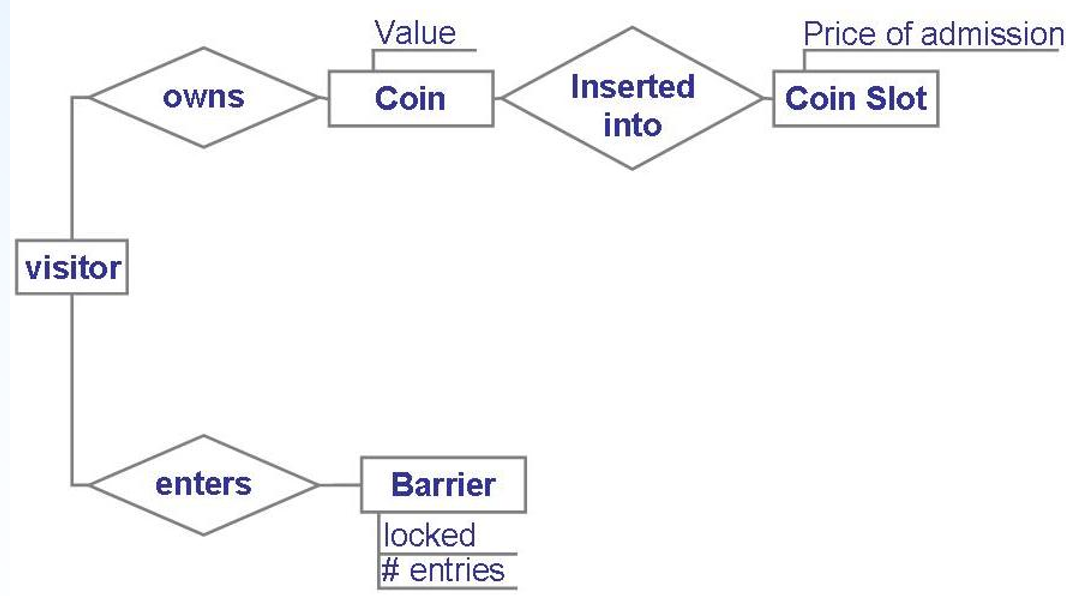
\includegraphics[scale = 0.3]{assets/SoftwareEngineering_86691.png}
    \caption{ER图,方框表示实体,菱形表示关系}
  \end{figure}
  \item 统一建模语言 UML

  \item 事件跟踪(时序图,协作图)
  \item 状态机
  \item Petri 网
  \item 数据流图(用例图)
\end{itemize}

\subsubsection{原型化需求}
使用原型来描述需求,容易回答用户界面的问题

\subsection{概要设计}
任务:根据SRS建立目标软件系统总体结构、设计全局数据库和数据结构,规定设计约束,制定集成测试计划等

技术途径和工具:自顶向下,逐步求精,抽象,模块化,局部化,信息隐藏等技术

阶段性产品:概要设计规格说明书,数据库或数据结构设计说明书,集成测试计划

\subsection{详细设计}
任务:细化概要设计所生成的各个模块,并详细描述程序模块的内部细节(算法,数据结构等) , 形成可编程的程序模块,制定单元测试计划

技术途径:根据SRS和概要设计结果进行,单入口单出口,PDL

阶段性产品:详细设计规格说明书,单元测试计划

\subsection{实现}
任务:根据详细设计规格说明社编写源程序,并对程序进行调试和单元测试,验证程序与详细设计文档一致性

阶段性产品:源程序代码

\subsection{集成测试}
任务:根据概要设计规格说明书,将经过单元你测试的模块逐步进行继承和测试

阶段性产品:生产满足概要设计要求、可运行的系统源程序和系统继承测试报告

\subsection{确认测试}
任务:根据软件需求规格说明书,测试软件系统是否满足用户需求

阶段性产品:可供用户使用的软件产品(文档,源程序)

\subsection{软件维护}
任务:对使用后的软件进行维护

阶段性产品:版本更新的软件产品

\section{软件过程模型}
\begin{itemize}
  \item 70-90年代,软件工程从无到有,以瀑布模型,结构化开发方法为主
  \item 90年来以来,以面向对象开发方法为主,重点为复用技术,构件,UML技术\\
  构件$\to$中间件$\to$体系结构
\end{itemize}

软件过程模型的目的:使软件开发有序

软件开发模型是软件开发全部过程、活动和任务的结构框架,他能直观表达软件开发全过程,明确规定要完成的主要活动、任务和开发策略

软件开发模型也常称为软件过程模型,软件生存期模型,软件工程泛型

\subsection{瀑布模型}
\begin{itemize}
  \item 软件过程的第一个模型
  \item 重量级模型
  \item 1970
  \item 把软件开发过程划分成多个阶段,描述各个阶段的关系,每个阶段在上一个阶段完成之后才能进行
  \item 从高到低像瀑布一样,因此叫瀑布模型
\end{itemize}

瀑布模型的特点:(推迟开发的观点)
\begin{itemize}
  \item 死板,严格按阶段,按顺序进行
  \item 对文档的要求高,每个阶段都提供文档\\
  历史原因:当时软件开发十分混乱,希望尽可能严格进行,有效的方法就是文档
  \item 严格有序地进行,用户要在最后阶段才能看到成品\\
  若产品与用户期望不一致,将是一个致命的问题
  \item 对于需求明确的软件,瀑布模型会是一个很有用的模型
  \item 采用结构化方法(当时还没面向对象)
\end{itemize}

优点:从一个非常高层次的角度描述开发过程中的活动,提出了要求开发人员经过的事件序列
\begin{itemize}
  \item 采用规范的方法,严格规定每个阶段提价的文档,要求每个阶段交出的产品必须经过验证\\
  分阶段 + 文档 + 验证
  \item 适合用户需求明确的开发
\end{itemize}

缺点:PPT
\begin{itemize}
  \item 没有循环、迭代
  \item 不适合需求变化的软件开发\\
  对如何处理开发中产品和活动的变化没有提供相关的直到
  \item 瀑布模型是由文档驱动的
  \item 将软件开发视为制造而不是创建
  \item 需要很长时间的等待
\end{itemize}

\textbf{怎么评价文档驱动的开发?}文档驱动既是优点也是缺点,文档过多 , 会增加时间成本

\textbf{原型化瀑布模型}
建立原型,原型也采用瀑布模型开发

\textbf{变种V模型}
引入测试(单元测试,系统测试和验收测试)
\begin{figure}[H]
  \centering
  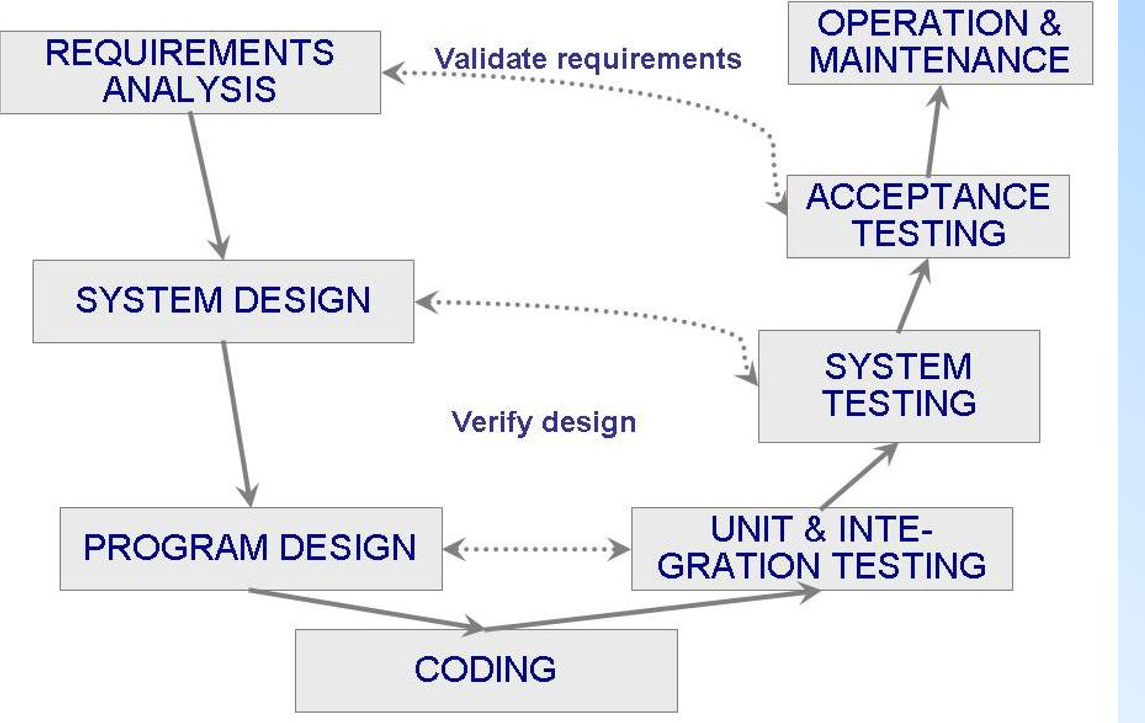
\includegraphics[scale = 0.3]{assets/SoftwareEngineering_50540.png}
  \caption{V模型}
\end{figure}


\subsection{原型化模型}
动机,适合情况:当难提出完整明确的需求,那么就先做一个完整的原型,从而让客户提出更具体明确的需求

提出背景:出现了快速搭建原型的工具

优点:允许需求或设计反复调查,减少开发中的风险和不确定性

对于原型,有两种处理方式(时间成本不同,处理方式不同)
\begin{itemize}
  \item 放弃原型,重新开发\\
  求块,不考虑质量
  \item 在原型的基础上,继续开发(演化模型)\\
  相对慢,遵循一定质量要求
\end{itemize}

原型法的关键是:怎么快速构造出原型

原型法的目的是:明确需求分析阶段

\subsection{可操作规格说明}
背景:对文档过程的管理,过于口语化;使用自然语言描述,可能导致对需求连接的不一致 $\to$ 能否通过数学化的方法描述

方式:定义一些关键词 、 语法

存在的问题:遵循特定的语法,可能没法广泛接受和使用

\subsection{增量和迭代}
阶段化开发方法:增量和迭代方法 , 当今互联网公司的主要方法

背景:即使是原型,也不能完全确定需求,因此瀑布模型不再合适

方法:把软件开发分成几期,每期做部分功能

\begin{itemize}
  \item 增量\\
  每次在原基础上增加部分功能,图4-3\\
  注:增量选择并非随意
  \item 迭代开发\\
  在原基础上,不断循环优化\\
  一开始提交完整的系统,再在每一期的发布中改变每个子功能的功能
\end{itemize}

优点(原因):
\begin{itemize}
  \item 即使缺少某些功能,也可以在早起的发布中就可以开始进行培训
  \item 可以及早为哪些以前从未提供的功能开拓市场
  \item 经常性的发布可以是开发人员全面、快速修复这些问题
  \item 开发团队将重点仿造不同的专业领域技术上
\end{itemize}

\subsection{螺旋模型}
螺旋模型:结合开发活动和风险管理,以将风险减到最小并加以控制(风险驱动)
主要围绕4个活动:计划、确定目标,可选方案,约束、评估可选方案和风险、开发和测试

\subsection{其他模型}
\begin{itemize}
  \item 喷泉模型\\
  基于面向对象方法开发
  \item 可重用组件组装模型
\end{itemize}

\subsection{敏捷软件过程}
敏捷软件过程:轻量级开发方法,强调迭代与代码规范化(减少文档,把部分内容转换移入代码中)

敏捷过程将整个软件生命周期分解为若干个小的迭代中期,通过每个迭代周期结束时的交付阶段性成果获取切实有效的客户反馈

2大特征:课本P46
\begin{itemize}
  \item 适应性
  \item 对人的关注
\end{itemize}

敏捷方法:强调灵活性在快速有效开发软件中的作用
\begin{itemize}
  \item 相对于过程和工具,更强调个人和交互的价值\\
  瀑布模型用户只有在需求与验收中出现
  \item 更喜欢在生产运行的软件投入时间,而非文档的编写
  \item 注重客户的合作,而非合同谈判
  \item 专注于对变化的反映,而不是创建一个计划而后遵循这个计划
\end{itemize}

敏捷原则:
\begin{itemize}
  \item 开发人员最优先要做的是通过尽早且持续地交付有价值的软件从而使客户满意
  \item 即使到了开发后期,也欢迎改变需求,敏捷过程利用变化为客户创造竞争优势
  \item 经常性地交付可以工作的软件
  \item 在整个项目开发期间,业务人员和开发人员必须天天都在一起工作
  \item 围绕被激励起来的个体构件项目为开发人员提供所需的环境和支持,并且新人他们能完成工作
  \item 在团队内部,最具有效果并富效率的传递信息的方法就是面对面的交谈
  \item 工作的软件是首要的进度度量标准
  \item 敏捷过程提倡可持续的开发速度,责任人,开发人员和用户应该能够保持一个长期且恒定的开发速度
  \item 不断地关注优秀的技能和好的设计会增强敏捷能力
  \item 简单是最根本的
  \item 最好的构件、需求和设计出自于组织团队
  \item 每隔一定时间团队会在如何才能更有效地工作方面进行泛型,然后相应地对自己的行为进行调整
\end{itemize}

\subsubsection{敏捷开发方法实例}

\begin{itemize}
  \item 极限编程 XP

  4个要点:
  \begin{itemize}
    \item 交流
    \item 简单\\
    表面:简单,设计简单,编码简单,注释简单及测试简单\\
    核心思想:专注于当前用户需求,不关心未来可能的变化
    \item 反馈
    \item 勇气
  \end{itemize}

\item 结对编程\\
2个人共用一台电脑,一个看一个写

\item 测试先行\\
一般是先编码在测试,测试先行则是在编码之前,先把测试用例完成(即编码的目的是为了使测试通过)
\end{itemize}

\subsection{其他敏捷过程模型}

\begin{itemize}
  \item ASD 自适应软件开发
  \item scrum
  \item 动态系统开发方法 DSDM
  \item crystal
  \item 特征驱动开发 FDD
  \item 敏捷建模 AM
  \item 敏捷统一过程 AUP
\end{itemize}

\subsection{软件能力成熟度模型,CMM}
之前侧重过程本身的规范化管理,CMM结果的评估和认证

CMM的5级阶段,一般为逐级认证:
\begin{figure}[H]
  \centering
  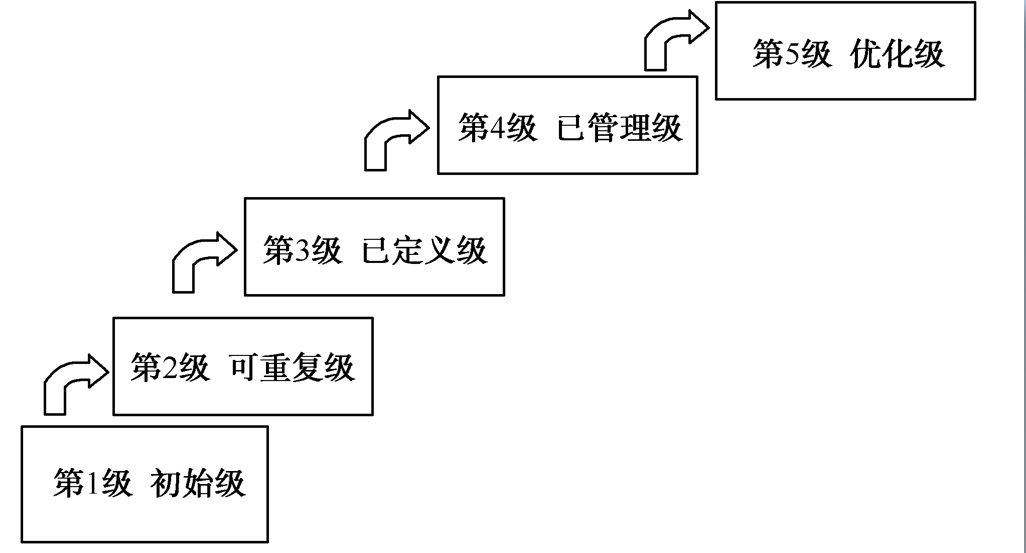
\includegraphics[scale = 0.3]{assets/SoftwareEngineering_c1bf0.png}
  \caption{CMM的5级模型}
\end{figure}

\begin{itemize}
  \item 初始阶段:过程无序且不可见,软件过程的特点是无秩序,有时甚至是混乱的
  \item 可重复:里程碑可见,按计划开发
  \item 已定义:每个阶段的内部活动可见,形成了整个软甲你组织的标准化软件过程
  \item 已管理:过程可质量,预测值与结果之间的偏差可控
  \item 已优化:过程动态调整,以及新技术的采用
\end{itemize}

\subsection{软件开发方法}

\begin{itemize}
  \item 结构化开发方法 \\
  70年代末以来,面向数据流的开发方法,本质为功能分解和抽象\\
  结构化方法包括:结构化分析(SA),结构化设计(SD),结构化程序设计(SP)
  \item 面向数据结构的软件开发方法
  \item 面向对象软件开发方法,20世纪90年代以来的革命性软件技术
\end{itemize}

\textbf{结构化与面向对象的区别?}\\
解决问题分为两个阶段:问题分析,求解(编码)

问题分析中,结构化与面向对象都采用相同的层次化的思想,都是自顶向下逐层细化问题。\\
而两者的区别主要在于编码部分,结构化采用自底向上的编码方式,而面向对象则是采用从中间向两边编码的方式。

\section{UML}
UML:一种建模语言,是为软甲系统的制品进行描述、可视化、构造、文档化的一种语言

4+1视图:视图由一种或多种模型图构成
\begin{itemize}
  \item 用例视图\\
  用例视图用来支持软件系统的需求分析,它定义系统的边界,关注的是系统的外部功能的描述\\
  从使用者的角度描述系统的外部静态功能和动态行为
  \item 逻辑视图\\
  定义系统的实现逻辑,描述为实现用例图描述的功能,在对软件系统进行设计时所产生的设计概念
  \begin{itemize}
    \item 设计视图
    \item 进程视图
  \end{itemize}
  \item 实现视图\\
  当系统的逻辑结构在逻辑视图被定义后,需要定义逻辑结构的物理实现
  \item 分布视图\\
  用来描述软件产品在计算机硬件系统和网络上的安装、分发、分布
\end{itemize}

\begin{figure}[H]
  \centering
  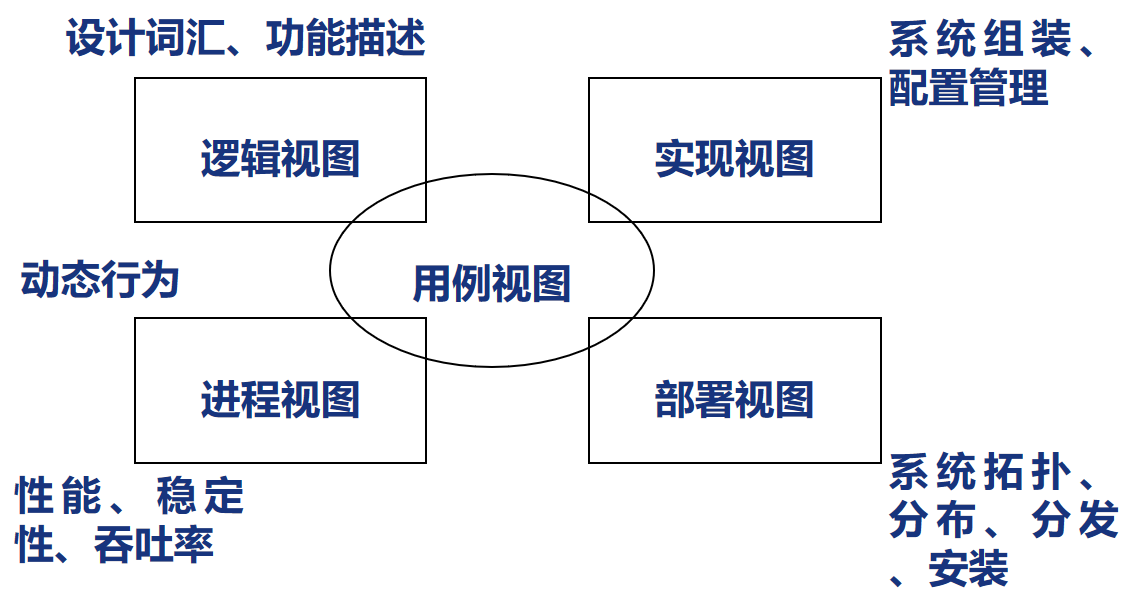
\includegraphics[scale = 0.3]{assets/SoftwareEngineering_7aecd.png}
  \caption{4+1视图}
\end{figure}

UML构成主要分3个方面:
\begin{itemize}
  \item 基本图素\\
  基本元素,如类,对象,包,接口,组件等
  \item 模型图\\
  用例图,类图,对象图等
  \item 建模规则
\end{itemize}

\textbf{UML基本模型元素分类:}结构模型元素 + 行为模型元素 + 分组模型元素 + 注解元素

结构模型元素:类,接口,协同,用例,主动类,组件,节点

行为模型元素:交互(多对象的行为)+状态机(单个对象自身状态的变化)

分组模型元素:模型包 package

\textbf{4种关系:} 关联关系(相互存在) + 依赖关系(单向) + 泛化 + 实现关系(比如:类与接口)

泛化:一般表现为继承关系,但泛化实际范围更广,它不要求两者之间有某种继承,只需要是特殊和一般的对比即可

\textbf{9种模型图:}类图,对象图,用例图,序列图,协同图,状态图,活动图,组件图,分布图

也有说分10种,第10种是包图,它实际上是作用于前9种图使得更方便管理


\textbf{UML的建模规则:}名字,作用域,可见性,完整性,运行属性

\textbf{UML公共机制:}规则说明 + 通用划分(类/对象) + 修饰 + 扩展机制

\textbf{UML的三种扩展机制:}
3个组成成分:
\begin{itemize}
  \item 构造型 stereotype:构造新的元素\\
  在图形名称上 , 使用双尖括号包围构造型
  \begin{figure}[H]
    \centering
    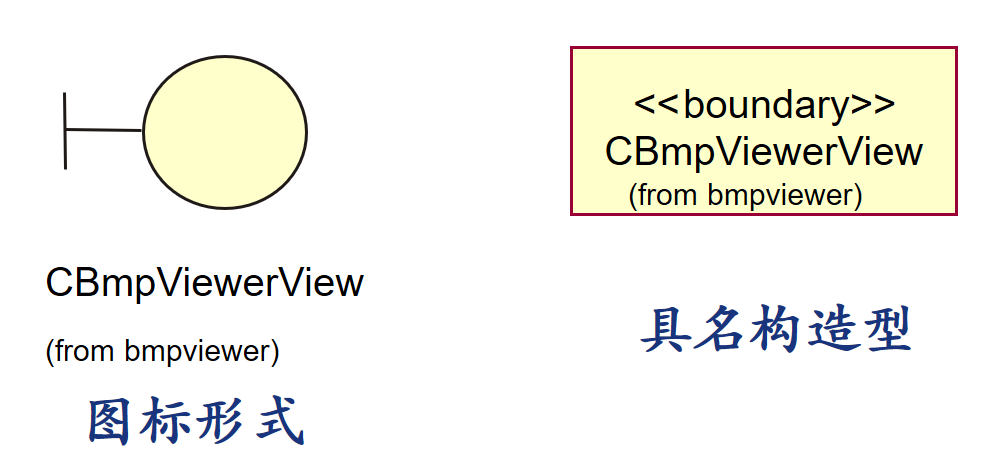
\includegraphics[scale = 0.3]{assets/SoftwareEngineering_1f53c.png}
    \caption{构造型两种表示方式}
  \end{figure}
  \item 标记值 tagged value\\
  构造型元素的属性(这个属性是更一般的属性,不一定是对象自身的特性,比如 版本号)\\
  使用花括号包围,放在名字下方
  \item 约束 contraint\\
  使用花括号放在箭头上
\end{itemize}

\subsection{用例图}
用例图:面向对象进入第二阶段的标志

用例图在需求分析阶段给用户的需求进行可视化,代表是的交互的过程,而不是步骤

组成部分:执行者 + 边界系统 + 用例

执行者与用例的关系:唯一的 ,关联关系 , 箭头的方向表示主被动关系

什么是用例?怎么样描述用户关心的事情?
\begin{itemize}
  \item 用例是从用户的角度对用户关心的事情的描述,不反映功能的实现方式
  \item 用例图的粒度具体到一个用户的目标
\end{itemize}

\begin{figure}[H]
  \centering
  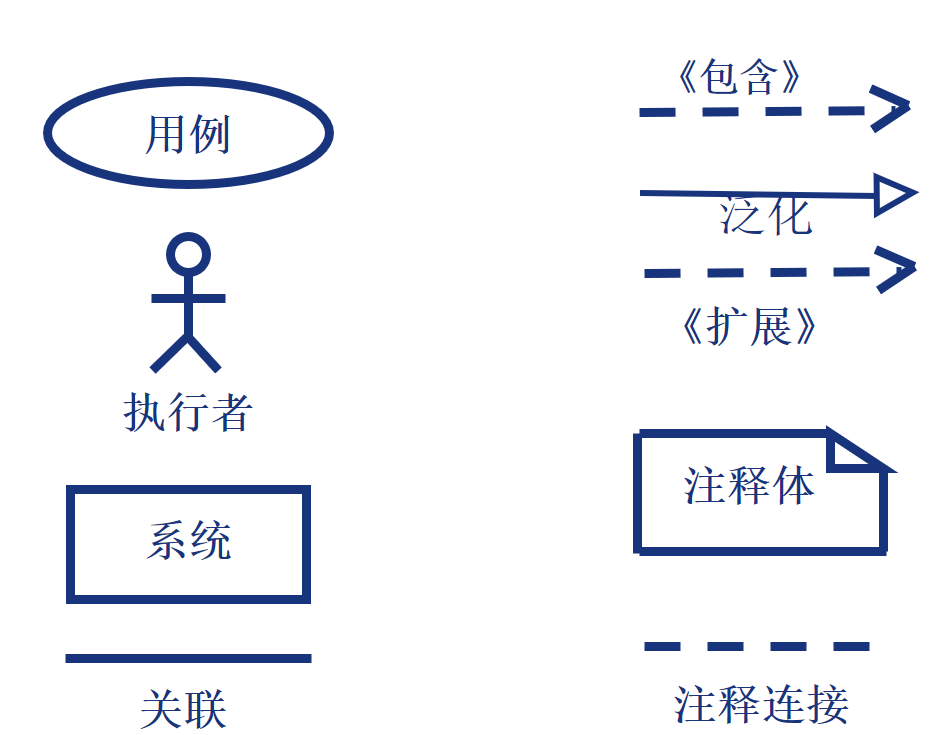
\includegraphics[scale = 0.3]{assets/SoftwareEngineering_ca369.png}
  \caption{用例图的图符}
\end{figure}
\begin{itemize}
  \item 执行者:执行者可以通过泛化关系来描述重叠的责任
  \begin{figure}[H]
    \centering
    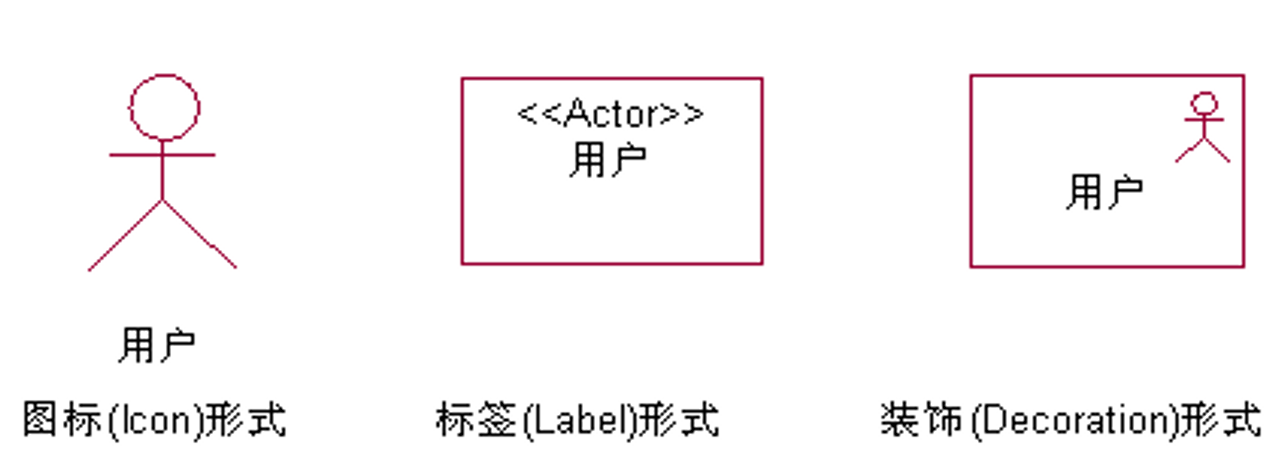
\includegraphics[scale = 0.3]{assets/SoftwareEngineering_fe408.png}
    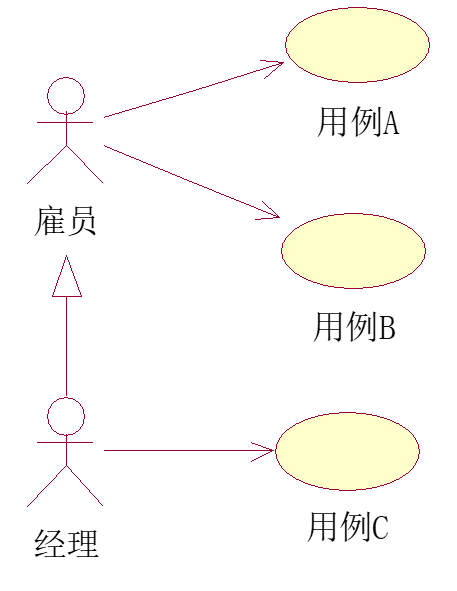
\includegraphics[scale = 0.3]{assets/SoftwareEngineering_8aab7.png}
    \caption{执行者的3种表示和泛化关系}
  \end{figure}
  \item 用例:用客户或用户的语言或词汇来描述的系统的一个完整功能
  \item 泛化:一般指同一功能的不同实现,一般与特殊的关系,A指向B,表示A继承自B
  一般子类默认接受来自父类的关系
  \item 关联:连接执行者和用例,关联关系上的数目表示实例化对象之间的数目关系
  \item 包含:由用例A连向用例B,表示A使用了B的行为或功能\\
  指一个功能包含另一个功能,这个功能一般是不同用例时间出现的公共的行为\\
  包含关系更强调复用,但是直接用来列举步骤也没毛病,但是不合理(即不要把每个步骤都表示成用例)\\
  其次,尽量避免包含关系的嵌套
  \item 扩展:由用例A连向用例B,表示B描述了一项基本需求,而A描述了该基本需求的一个特殊情况\\
  可以看成是条件执行,B指向A,表示B扩展出A,B为A某种特殊情况发生才执行的用例(箭头由特殊指向一般)\\
  当有多个拓展关系的时候,把扩展节点描述在线上
  \begin{figure}[H]
    \centering
    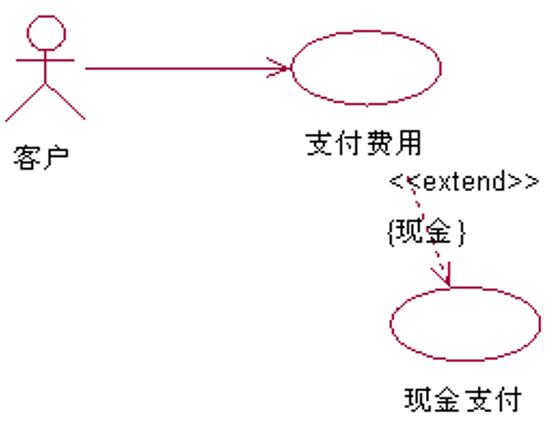
\includegraphics[scale = 0.3]{assets/SoftwareEngineering_5d2ad.png}
    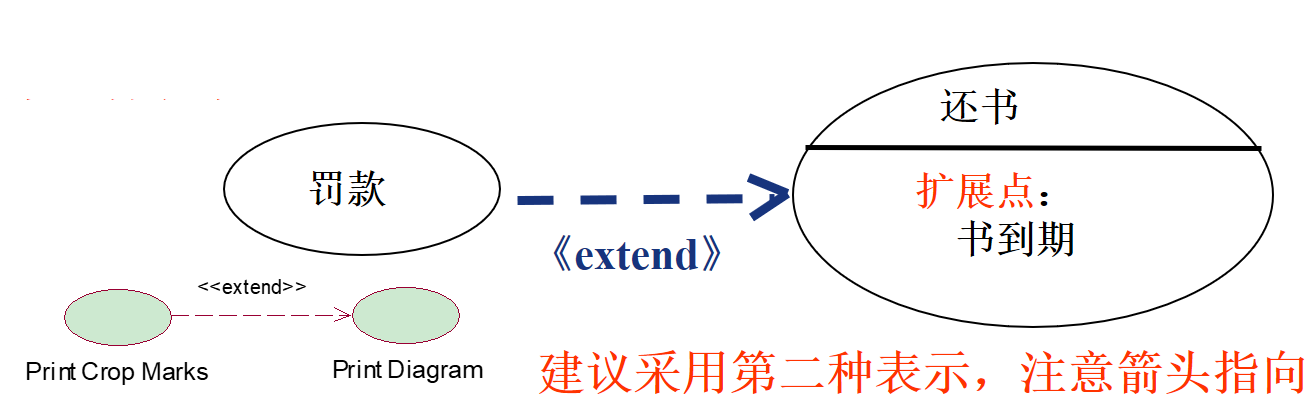
\includegraphics[scale = 0.3]{assets/SoftwareEngineering_0b9db.png}
    \caption{扩展关系的两种表示}
   \end{figure}
\end{itemize}
\spaceline

\textbf{执行者与用例之间的关系}:只有唯一的关联关系
主要的地方在于连线的箭头的方向,表示主被动的关系,当主被动关系不明确,或者相互的时候,则无箭头


\subsubsection{包含和扩展关系}

包含:当一个通用的用例可以成为几个特殊的用例的组成部分时用包含关系。因此,当在两个或更多的用例中出现重复描述而又想避免这种重复时,采用包含关系。

扩展:当一个用例是另一个一般化用例的特例时,用扩展关系。因此,当描述一般行为的变化时,采用扩展关系。

\begin{figure}[H]
  \centering
  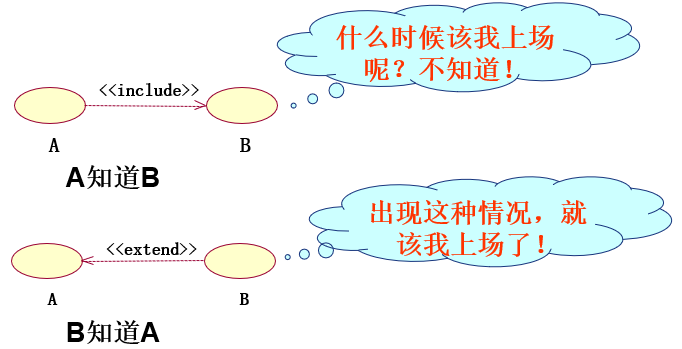
\includegraphics[scale = 0.3]{assets/SoftwareEngineering_7ddd5.png}
\end{figure}

扩展和包含用例本质上其实非常相似,它们的主要区别在于用例实例中断基用例、执行附加用例的方式

\subsubsection{扩展与泛化的区别}
\begin{itemize}
  \item 泛化关系的双方之间有内在的相同的东西
  \item 可以表示成泛化关系的双方也可以表示成扩展关系,反过来则不一定
\end{itemize}

\subsubsection{建立用例模型的主要工作}
建立用例模型的主要工作:
\begin{itemize}
  \item [1.]定义系统
  \item[2.]找出执行者
  \item[3.]找出用例
  \item[4.]描述用例
  \item[5.]用例的整理与加工
  \item[6.]验证模型
\end{itemize}

一般情况下,执行者放在系统边界的两边,主动的放左边,被动的放右边,上下一般留空。

\subsubsection{用例图的作用}
用例图用来描述软件续期模型中的系统功能,通过一组用例可以描述软件系统能够给用户提供的功能

用例图可以作为整个系统开发过程中的开发依据,指导和驱动其他模型

\section{类图}
类图:描述逻辑概念上的关系

类图主要包含两类元素和4种关系

两类元素:\textbf{接口} , \textbf{类}

类图包含4种关系:关联 + 实现 + 依赖 + 泛化

类图的作用:描述类、接口之间的关系

类图用在哪个阶段?系统的设计阶段

类图体现静态结构

\textbf{类的层次结构:}
\begin{itemize}
  \item 层次过多$\to$结构复杂
  \item 层次过少$\to$复用性弱
  \item 一般建议6-7层
\end{itemize}

\begin{figure}[H]
  \centering
  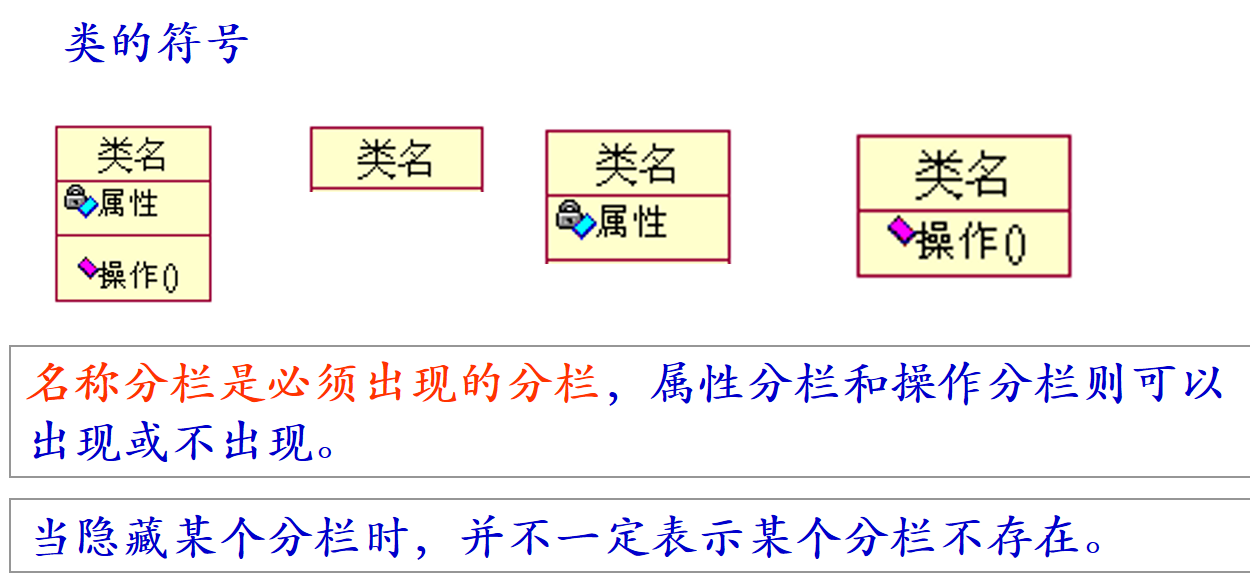
\includegraphics[scale = 0.3]{assets/SoftwareEngineering_ce110.png}
  \caption{类图的符号表示:属性、操作是可选项,类名 必选}
\end{figure}
图形未显示并不代表一定没有属性,可能隐藏了一些不重要属性

\textbf{名字加下划线:}
\begin{itemize}
  \item 名称下加了下划线,表示具体对象
  \item 属性加下划线 , 表示静态属性
  \item 方法加下划线 , 表示静态方法
\end{itemize}

\textbf{名字为斜体}
\begin{itemize}
  \item 类名为斜体, 表示抽象类
  \item 方法斜体, 表示抽象方法
\end{itemize}

类图和对象图的基本要素:关联,属性,操作,泛化,授权,约束规则

\subsection{关联}

关联:表示多个对象之间的结构关系

\textbf{关联关系符号:}实线,线上数字表示多元性,线上填关联的名称,线的源端和目标端表示角色

\begin{figure}[H]
  \centering
  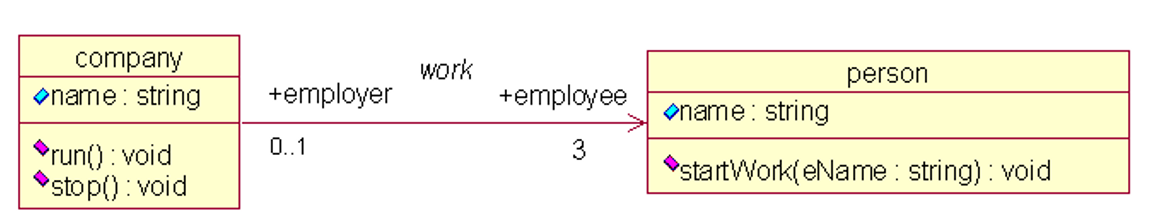
\includegraphics[scale = 0.3]{assets/SoftwareEngineering_9a276.png}
\end{figure}

\subsection{属性}

\textbf{属性}:
\begin{itemize}
  \item 可见性:公(+),私(-),保护(\#)
  \item 名称
  \item 多重性:0..*
  \item 类型
  \item 缺省值
  \item 约束特性
\end{itemize}

\subsection{操作}
操作:描述类的行为的函数,包括可见性, 参数表 ,返回类型(可选)

符号表示:可见性 名称(参数表):返回类型

\subsection{泛化关系}
继承与泛化的关系:继承是泛化的一种实现机制,但并非所有的泛化关系都适合用继承关系实现

泛化关系的应用:多态 , 父类所定义的操作被子类继承后可以表现出不同的行为(子类覆盖父类的同名方法)

符号表示:实线+ 空心箭头,箭头含义:A$\to$B表示A继承自B

\subsection{类间关系:组合聚合}
\begin{itemize}
  \item 聚合\\
  空心菱形,表示整体与部分的关系\\
  从代码的角度来看,"整体"释放之后, 不用理 "部分"的声明周期\\
  聚合的成分脱离整体之后依旧可以独立存在 PPT87-89
  \item 组合\\
  实心菱形 , 组合是聚合的一种\\
  整体-部分的声明周期相同
\end{itemize}

符号描述:在整体端加菱形,另一端为普通箭头
\begin{figure}[H]
  \centering
  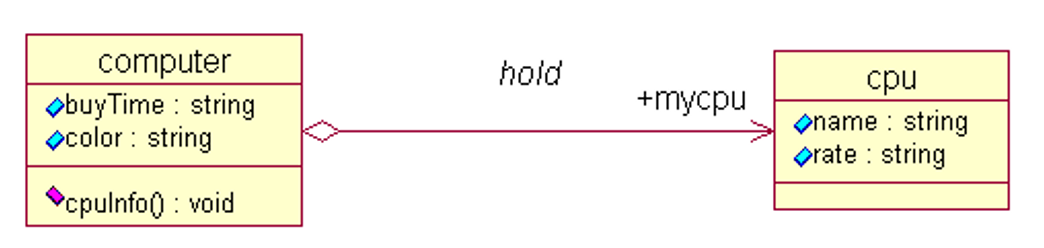
\includegraphics[scale = 0.3]{assets/SoftwareEngineering_cbbbe.png}
\end{figure}

组合与聚合关系从语法上是没法区分的,从语义上才能更好地区分两者

\subsubsection{组合、聚合、关联}

组合/聚合与关联的区别:
\begin{itemize}
  \item 关联关系所涉及的两个类是处在同一个层次上的。
  \item 聚合关系涉及的两个类处于不平等的层次上,一个代表整体,一个代表部分。
\end{itemize}

聚合与组成的区别:
\begin{itemize}
  \item 组合:整体类端的重数必须是1,部分类的重数是任意的
  \item 聚合:整体类端的重数可以大于1,部分类的重数是任意的
\end{itemize}

\subsection{依赖关系}
$A-> B$:表示A依赖B, B的变化会引起A的变化

什么情况会产生依赖消息?
\begin{itemize}
  \item 一个类出席县在另一个类的对象,作为自己某个操作的参数
  \item 是操作的局部变量
\end{itemize}

\subsection{约束规则}
\textbf{约束规则语法:}放在 \textbf{\{\}}中,用断言作为实现


\subsection{对象图}
对象是类的实例,对象图可看做类图的实例,主要用于了解系统在特定时刻的具体情况,以求发现类图中的错误,进而修正类图

匿名对象:名字部分为空

\subsection{类图建模分析步骤}
\begin{itemize}
  \item 寻找出需求中的名词(候选对象)。
  \item 合并含义相同的名词,排除范围以外的名词,并寻找隐含的名词。
  \item 去掉只能作为类属性的名词。
  \item 剩下的名词就是要找的分析类(候选类)。
  \item 根据常识、问题域、系统责任确定该类有那些属性。
  \item 补充该类动态属性,如状态、对象间联系(如聚合、关联)等属性。
  \item 从需求中的动词、功能或系统责任中寻找类的操作(候选操作)。
  \item 从状态转换,流程跟踪、系统管理等方面补充类的操作。
  \item 对所寻找的操作进行合并、筛选。
  \item 对所寻找的操作在类间进行合理分配(职责分配),形成每个类候选操作。
  \item 补充每个类的的分析文档,为类的进一步设计打下基础。
\end{itemize}

\section{接口、抽象类}
抽象类:
\begin{itemize}
  \item 采用斜体表示抽象类的名称,或者用 \textbf{\{abstract\}  }
  \item 缺足够详细的信息来实例一个对象
\end{itemize}

\textbf{为什么引用 抽象类这个概念?而不是用普通类代替?}

随着编程易忘记某个类是抽象类的事实而误用,引用 \textbf{抽象类} 可避免这个问题从而提到代码质量


接口的符号:
\begin{figure}[H]
  \centering
  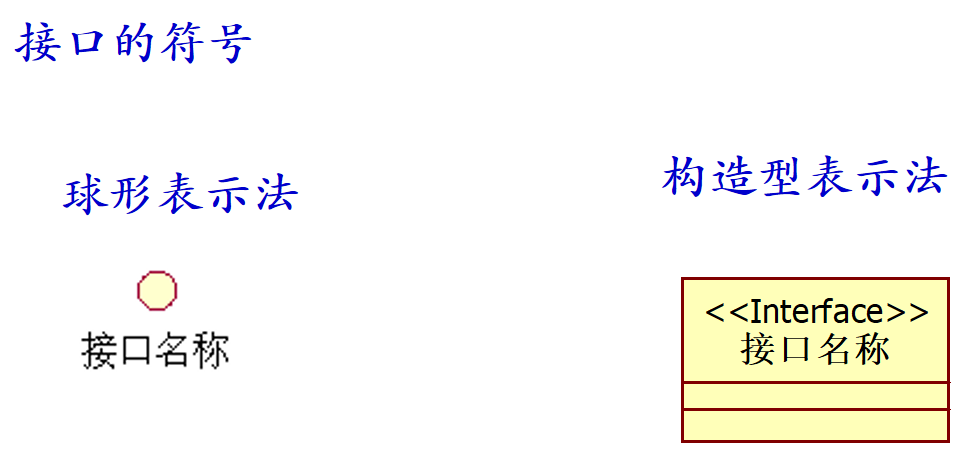
\includegraphics[scale = 0.3]{assets/SoftwareEngineering_22c0e.png}
\end{figure}

接口的特点
\begin{itemize}
  \item 接口中只包含普通函数,不包含构造函数
  \item 接口中只能提供方法的格式声明,而不能包含方法的实现
  \item 接口中的所欲函数都被视为公有,不需要添加可见性
  \item 一个类可以实现多个接口
\end{itemize}

接口之间能继承吗?背景:为解决只有单一继承下的多重继承问题

为什么需要接口?
\begin{itemize}
  \item 可以实现多继承
  \item 通过接口实现不相关类的相同行为,而无需考虑这些类之间的关系
  \item 通过接口知名多个类需要实现的方法
\end{itemize}

常量接口:java中会自动加上 static final public

接口与抽象类的比较:
\begin{itemize}
  \item 抽象类允许增加一些方法的实现,但接口必须推迟定义所有的方法
  \item 从语义的层面上,抽象类是一种类对一组具有相同属性和方法的逻辑上有关系的事物的抽象,而接口则是对一组具有共同属性和方法的逻辑上不相关的事物的一种抽象
  \item 抽象类可以有自己的数据成员,而接口内的数据成员只能是常量
  \item 一个类只能继承一次,而可实现多个接口
  \item 抽象类的方法有默认行为
\end{itemize}

\section{各种关联}
\begin{itemize}
  \item 限定关联
  \item 关联类
  \item 双向关联
  \item 单向关联
  \item 递归关联(反射关联)
\end{itemize}

\section{交互图}
\begin{itemize}
  \item 顺序图(时序图,序列图)
  \item 协作图\\
  在uml2.0 协作图改为通信图
\end{itemize}
序列图(顺序图)、协作图(通信图):表示动态行为 , 描述对象之间的关系,序列图和协作图在语义上等价


\subsection{序列图}
序列图:强调的是消息发送的时间的先后顺序

优点:简单直观

缺点:对象多时,浪费空间, 交互时不适合描述有选择、并发等复杂情况

序列图的表示:
\begin{itemize}
  \item 方框:激活期
  \item 虚线:生命周期\\
  结束虚线末端打叉
  \item 发送消息:$\to$
  \item 接收(返回)消息$-->$
  \item 临时创建对象:对象在下移的过程中出现
  \item 过程循序号,过程顺序号是嵌入的\\
  比如发送消息2,启动了其后的一些列消息,可以变好为2.1,2.2
  \item 条件:用中括号表示
\end{itemize}

\subsection{协作图}
对象多时,采用协作图,通过编号来表示顺序

协作图侧重于描述对象之间消息的连接关系

协作图对象用对象图符表示,箭头表示消息发送的方向,编号表示消息的执行顺序

\section{状态图}
状态图由状态机产生,用来描述对象内部的状态,用来描述一个对象在其生命周期中所表现出来的状态和行为

状态图由状态以及引起状态变化的外部事件组成

状态图的表示:箭头 , 源端表示起始状态,目标端表示目标状态,线上 : 触发时间名[触发条件]/变迁的动作

条件转移:使用菱形展开
\begin{figure}[H]
  \centering
  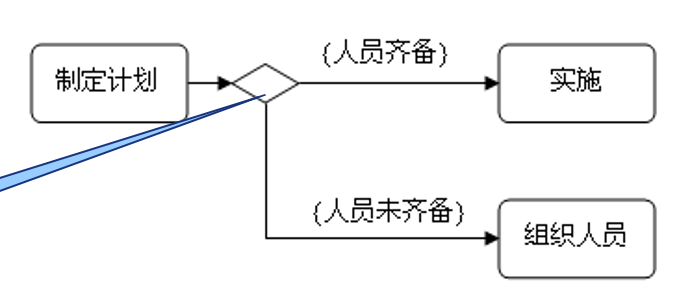
\includegraphics[scale = 0.3]{assets/SoftwareEngineering_e7bd4.png}
\end{figure}

\begin{figure}[H]
  \centering
  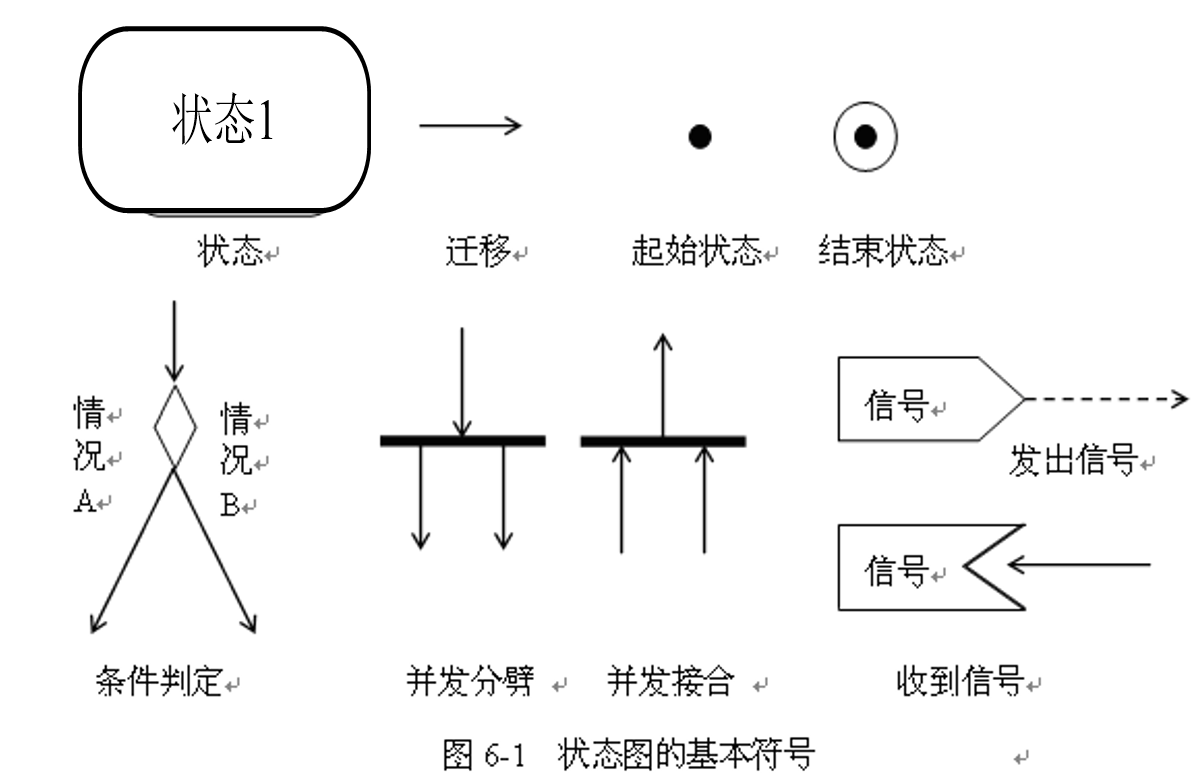
\includegraphics[scale = 0.3]{assets/SoftwareEngineering_a70d3.png}
  \caption{状态图的基本符号}
\end{figure}

\section{活动图}
活动图:类似流程图,是一种特殊形式的状态机



活动图在什么时候使用?在需求分析时

图符的含义的区别?
\begin{itemize}
  \item 状态图表示状态本身,活动图表示一个活动
  \item 活动的变迁无外部事件,状态图由外部事件驱动
  \item 活动图可能涉及多个对象
\end{itemize}

活动图的作用:描述控制在活动之间的流动,辅助需求分析

使用场景:
\begin{itemize}
  \item 业务流程
  \item 对象的特定操作建模
\end{itemize}

\begin{itemize}
  \item 活动图强调整个执行过程的步骤(活动以及活动之间的关系)
  \item 活动图强调多个对象之间是协作的
  \item 活动图和状态图的图符基本一致,但是图符的含义不同
  \item 状态图针对单个对象由外部事件驱动 , 而活动图状态的变迁不需要事件触发
\end{itemize}

活动图与状态图的区别?
\begin{itemize}
  \item 触发迁移的机制不同
  \item 描述多个对象共同完成一个操作的机制不同\\
  活动图通过泳道体现多对象,状态图涉及多个对象时可以用嵌套的形式表达,即一个对象由多个子对象组成
\end{itemize}

相同点:
\begin{itemize}
  \item 都是状态机的一种,描述一个系统或生存期间的状态或行为
  \item 图符基本相同
  \item 可以描述多进程操作中的同步或异步操作的并发行为
\end{itemize}

\subsection{泳道}
活动图通过泳道体现多对象,状态图涉及多个对象时可以用嵌套的形式表达,即一个对象由多个子对象组成

泳道:对活动按对象进行分组管理

对象流:虚箭头 , 一个活动可以有多个输入,多个输出

\begin{figure}[H]
  \centering
  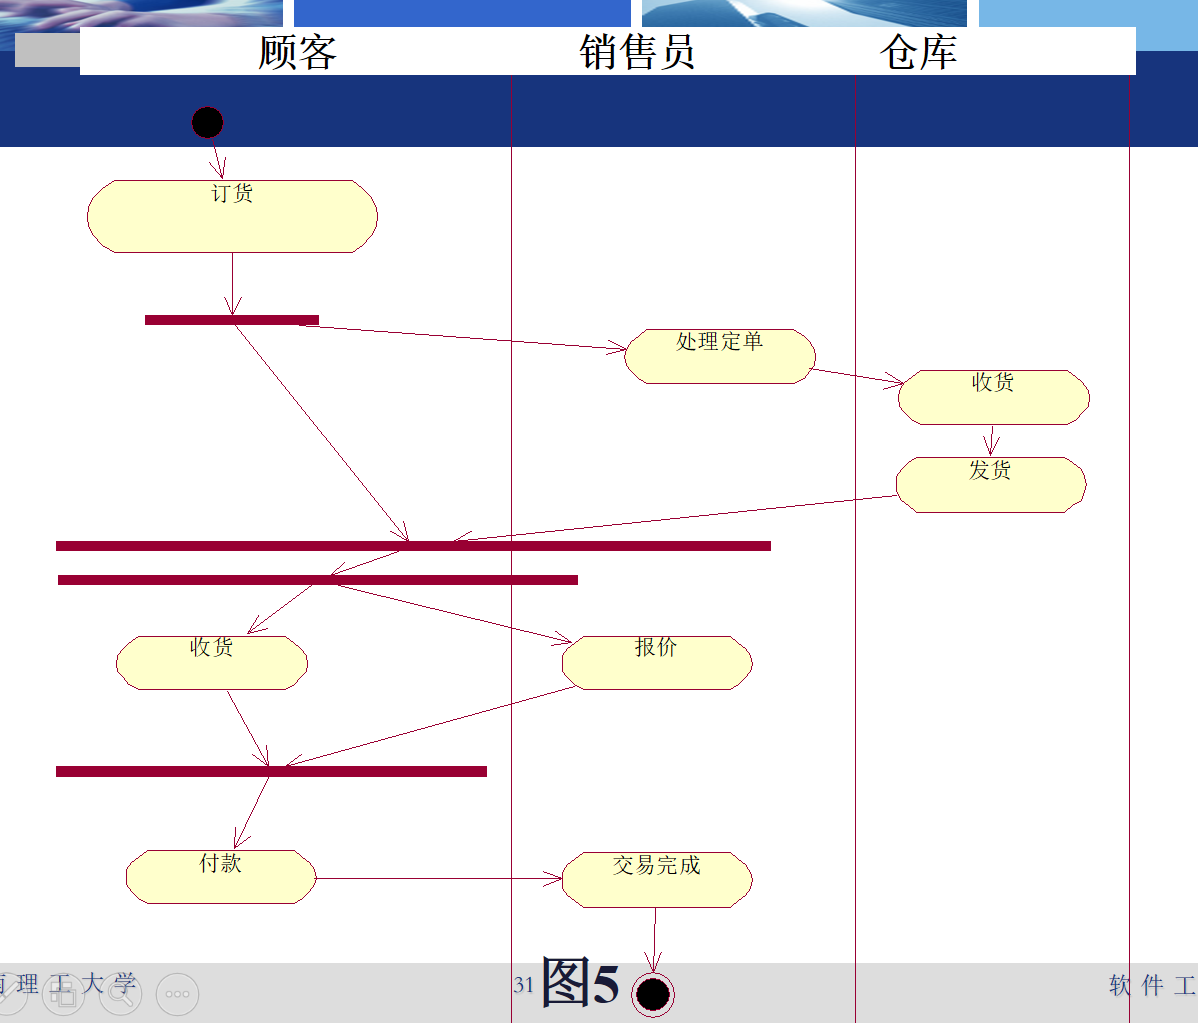
\includegraphics[scale = 0.3]{assets/SoftwareEngineering_f1548.png}
\end{figure}

\subsection{交互概览图}
交互概览图:活动图中的一个节点可能为交互图(在活动图中是引用,而非把整个图画上去)

交互概览图是活动图的一种

此时,交互概览图 , 加边框,左上边加关键词(添加可被引用的特点),引用的时候,左上角加"ref"

\begin{figure}[H]
  \centering
  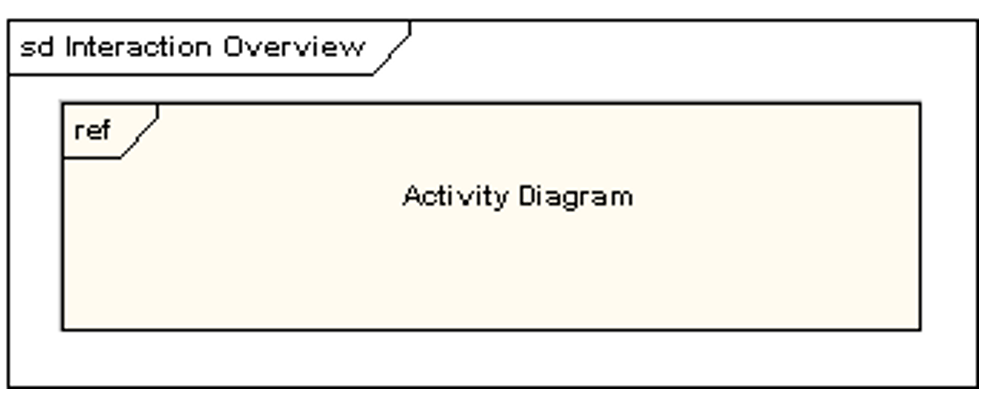
\includegraphics[scale = 0.3]{assets/SoftwareEngineering_c78cc.png}
\end{figure}

\section{组件图}
组件是物理存在的,如源代码,二进制文件等,组件通过接口对外提供声明

组件与接口的关系:实现与依赖关系

组件图:处于实现视图

\begin{figure}[H]
  \centering
  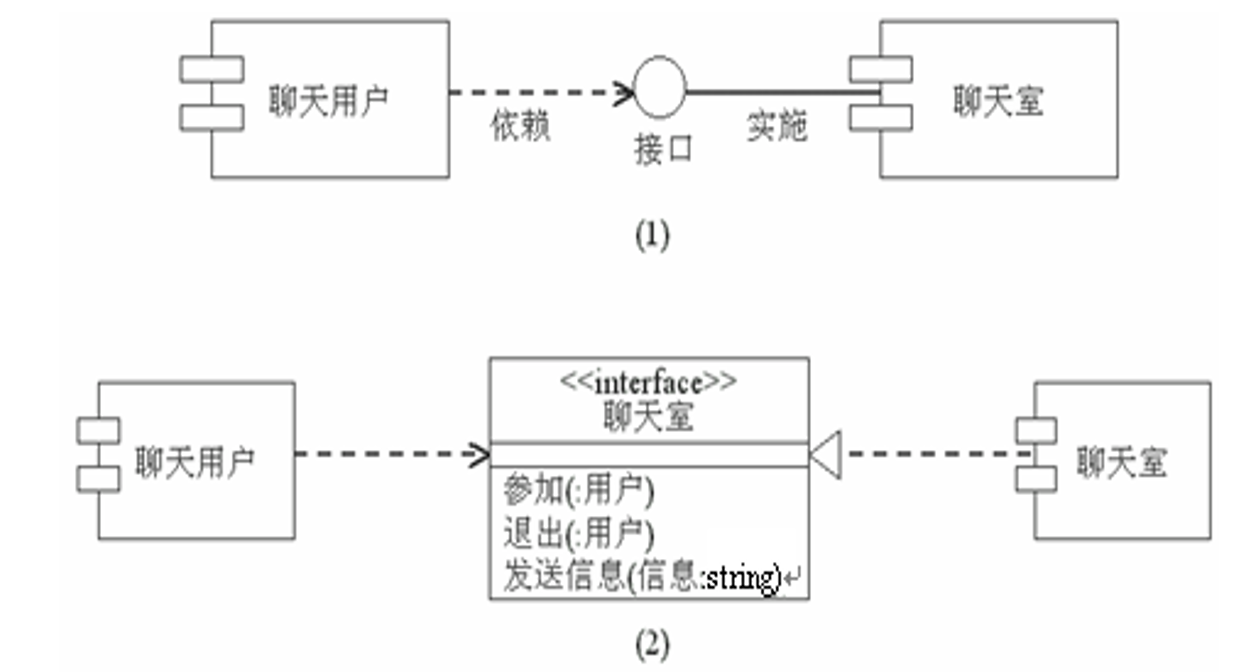
\includegraphics[scale = 0.3]{assets/SoftwareEngineering_ab4cf.png}
\end{figure}

\section{部署图}
部署图:描述节点和组件之间的关系,用来描述软件产品在计算机硬件系统和网络上的安装、分发、分布

节点指的是硬件资源,比如处理器和设备,处理器指带有一定的计算能力(CPU)而设备部具有计算鞥里,使用一个立方体来表示

组件表示软件资源

组件存在于物理资源上(存储/运行)

\begin{figure}[H]
  \centering
  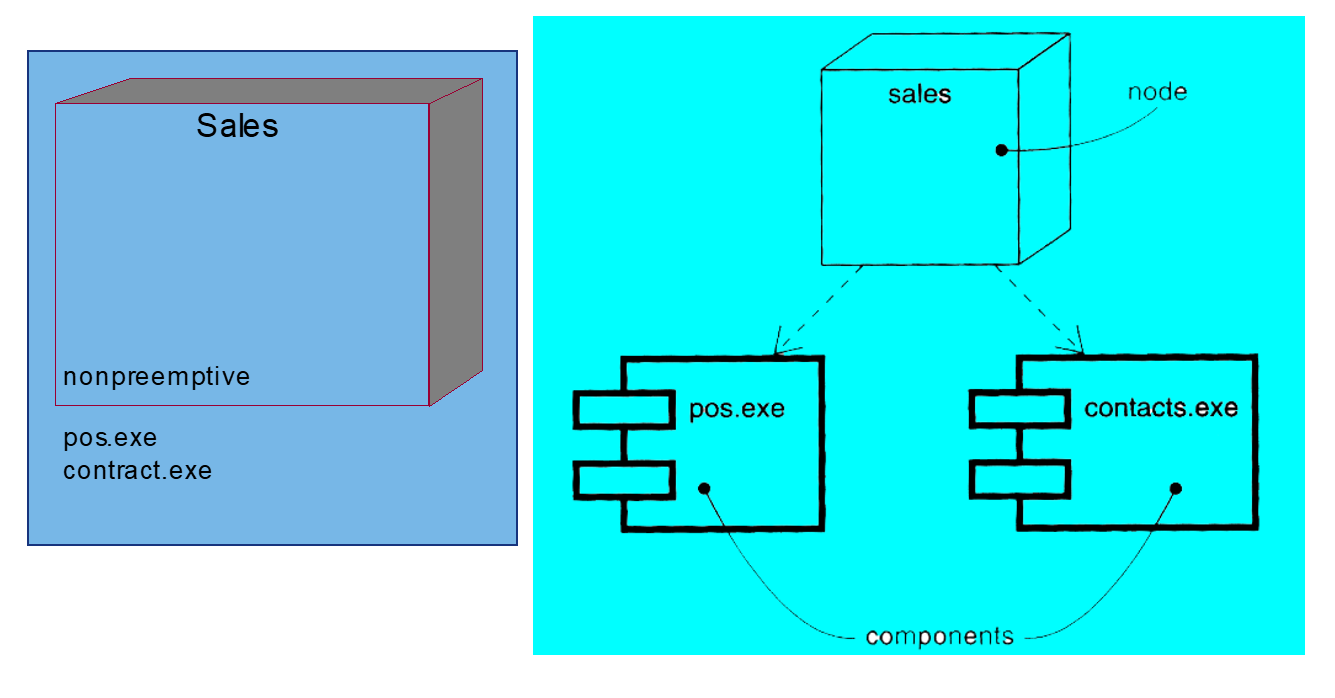
\includegraphics[scale = 0.3]{assets/SoftwareEngineering_8ff94.png}
\end{figure}

节点之间的关联关系,表示节点之间的物理连接

\subsection{小结}
UMP总共有9种常用图形,
我们通常使用4 + 1视图来理解

\begin{itemize}
  \item 用例视图\\
  描述做什么的问题
  \begin{itemize}
    \item 用例图
    \item 活动图
  \end{itemize}
  \item 逻辑视图\\
  描述如何做
  \begin{itemize}
    \item 静态结构
    \begin{itemize}
      \item 类图
      \item 对象图\\
      类图在某个时刻上的快照
    \end{itemize}
    \item 动态行为
    \begin{itemize}
      \item 交互图\\
      描述对象之间的外部行为
      \begin{itemize}
        \item 序列图
        \item 协作图
      \end{itemize}
      \item 内部状态
      \begin{itemize}
        \item 状态图
        \item 活动图
      \end{itemize}
    \end{itemize}
    \item 实现视图\\
    该视图在UML中没有体现
    \item 组件视图\\
    组件图
    \item 部署视图\\
    部署图
  \end{itemize}
\end{itemize}

\section{面向对象设计原则}
\textbf{对象 Object概念指的是什么?(历史起源?)}来自哲学,1922年$客观世界 \geq 事实 \geq 原子事实 \geq 对象$ , 在80,90年代引入计算机

\textbf{引入对象的原因?}
\begin{itemize}
  \item 背景:功能不稳定 ,实现方式不断变化
  \item 由对象来描述会相对稳定
  \item 符合我们认识客观世界的思路
\end{itemize}

\textbf{面向对象的3大特征:}封装 + 继承 + 多态

提出问题:可否把正方形作为长方形的子类?为什么?

不可以,虽然从数学的角度来看,正方形的确是长方形的一种特殊情况

采用PPT的实现,
以PPT的resize函数为例,<=,对于正方形,结果是横等于,那么程序将将入无限循环

那么,问题出现在哪(为什么子类对象使用在父类对象的地方会出现错误?)?如何避免这样的问题?怎么办?

模式设计的目标:
\begin{itemize}
  \item 可重用性
  \item 可扩展性
  \item 灵活性
  \item 可插入性
\end{itemize}

代码质量差的原因
\begin{itemize}
  \item 过于僵硬
  \item 过于脆弱
  \item 复用率低
  \item 粘度过高
\end{itemize}

常用的模式设计方法:
\begin{itemize}
  \item LSP 里氏替换原则\\
  任何父类可以出现的地方,子类也能出现->这就要求子类不能添加任何父类没有的附加条件,因为在以父类来进行代码编写的时候
  ,不会考虑父类没有的约束,从而导致代码存在风险
  \item OCP 开-闭原则\\
  开-闭原则,支持扩展而无修改原代码\\
  对扩展开放,对修改关闭
  \item SRP \\
  单一职责原则,一个接口尽可能单一几种
  \item ISP\\
  接口隔离原则,类间关系尽量用接口隔离,使用多个专门接口优于使用单一接口
  \item DIP\\
  依赖导致原则,应该具体依赖抽象,针对抽象(接口)编程,而不针对具体实现编程
  \item CRP,FCOI\\
  优先使用组合或聚合,不要过于使用继承关系
  \item LoD 迪米特原则\\
  一个软件实体对其他软件实体的引用越少越好
\end{itemize}

\subsection{里氏替换原则 分析 LSP}
LSP:任何父类能出现的地方子类也能出现

LSP描述类的关系

这要求子类不能添加约束,也就是说,使用子类实现复用则没问题,但是如果通过增加约束来派生子类则需要谨慎

PS:JAVA内置的LSP

不满足LSP的可能是以下原因:
\begin{itemize}
  \item 不构成父子类关系

  \item 有共同的父类
\end{itemize}

怎么做才能满足LSP?
\begin{itemize}
  \item 尽量不从具体类(非抽象类)继承
  \item 行为集中向上(抽象类)
  \item 数据集中向下(具体类)
\end{itemize}

\subsubsection{子类型和继承(子类)}

子类型(sub type)和继承(子类sub class / inheritance)的区别?

两者并不严格相等\\

子类型关系:最初的程序语言,语言的类型要求严格相等,这就造成了很大的不便,\\
比如在能使用实数的地方,使用整数也可以,但是因为类型不同的关系,导致无法使用\\
由此引入了"子类型的说法"

那么什么情况下构成子类型关系呢?\\
任何属于S的也属于T,那么S和T就构成了子类型关系\\
比如:任何属于int的也属于float

那么子类和子类型到底有什么区别呢?\\
\begin{itemize}
  \item 从子类型的定义可以看出子类型满足LSP,而子类则不一定满足LSP
  \item 继承是代码共享的一种重要途径,子类型是某种外部可观察行为(语义行为),与代码无关
\end{itemize}

\subsubsection{可替换性,协变 , 反变}
协变:covariant

反变:contravariant

两者共同的点是:都要求父类出现的方法必须在子类中出现。但是考虑到subtype的概念,
那么方法的结果(返回类型)和参数则不一定是完全一致的。

covariant考虑的是返回类型,子类的方法的结果可以比父类更广

contravariant考虑的是参数,子类的参数必须是父类的子类型

\begin{figure}[H]
  \centering
  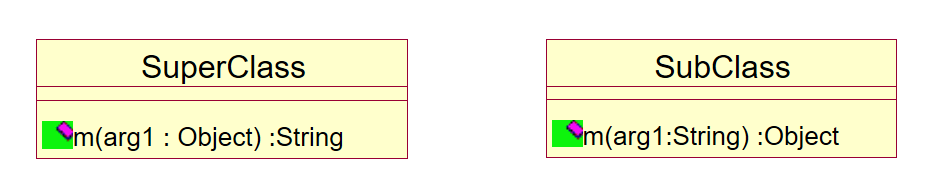
\includegraphics[scale = 0.3]{assets/SoftwareEngineering_b54a7.png}
\end{figure}

\subsection{OCP原则}
OCP原则:开-闭原则,对扩展开放,对修改关闭

OCP:描述目标

OCP原则的关键在于 抽象
\begin{itemize}
  \item 抽象预见了可能的所有扩展
  \item 由抽象可以随时导出新的类
\end{itemize}

\subsection{SRP原则}
SRP原则:单一职责原则,就一个类而言,应该仅由一个引起它发生变化的原因

具体的说,就是一个类尽可能只承担一个职责

SRP是高内聚低耦合的指导方针

\subsection{ISP}
ISP原则:接口隔离原则,用户不应该依赖他们不用到的方法,只给每个用户它所需的接口

这要求我们尽可能的使用小而精的接口

\subsection{DIP}
DIP描述类内关系

DIP,依赖导致原则,针对接口编程,不要针对实现编程

原本我们的分析是针对底层实现,逐渐向上依赖,而DIP原则则要求我们顶层和底层都依赖中间层

\begin{figure}[H]
  \centering
  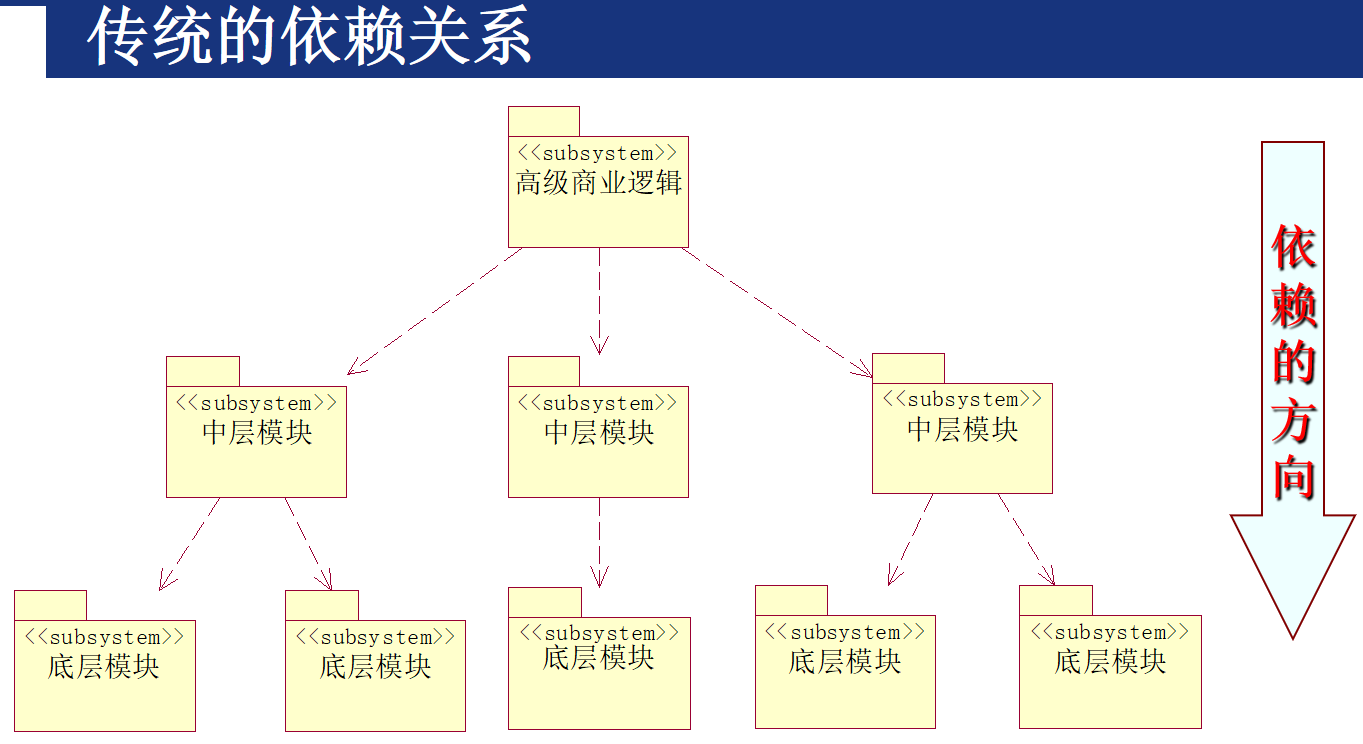
\includegraphics[scale = 0.3]{assets/SoftwareEngineering_17391.png}
\end{figure}

\begin{figure}[H]
  \centering
  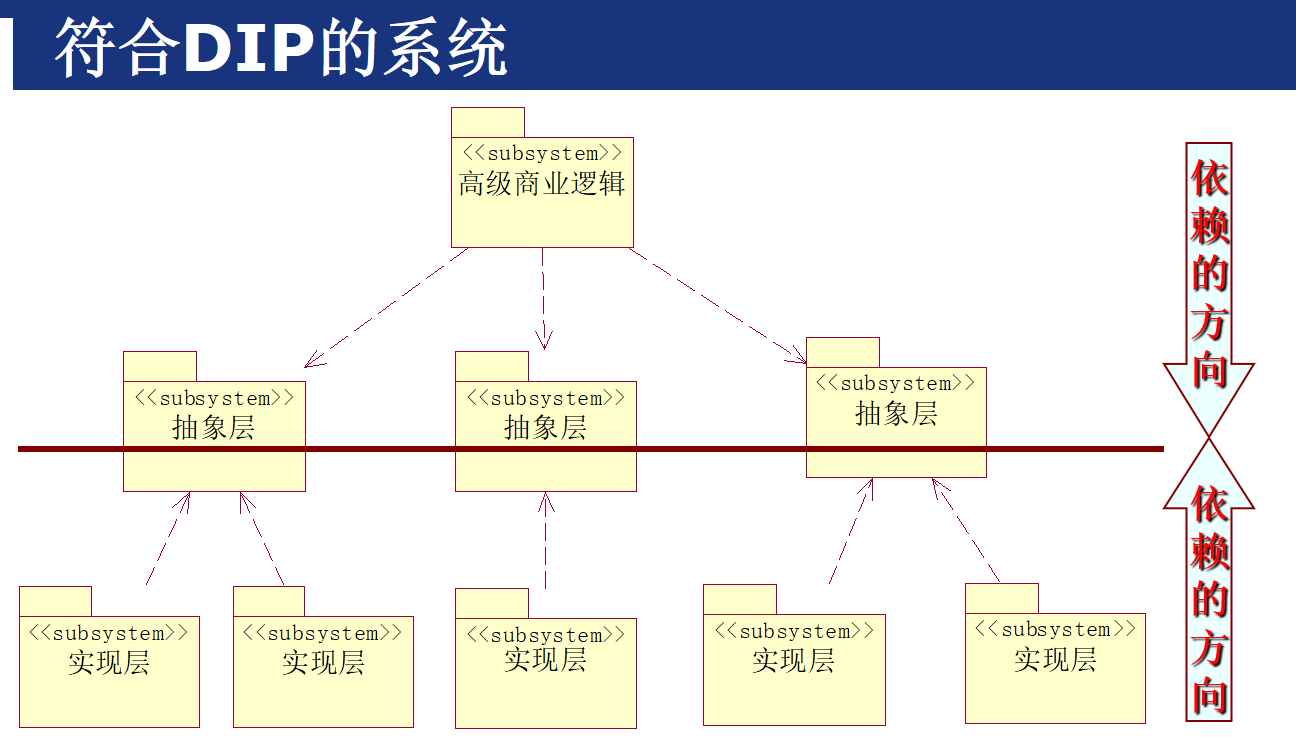
\includegraphics[scale = 0.3]{assets/SoftwareEngineering_dc683.png}
\end{figure}

\subsection{FCOI 组合复用原则}
优先使用组合而非对象,组合代表黑盒复用,对象代表白盒复用

继承复用的缺点:
\begin{itemize}
  \item 会破坏对象本身的封装性
  \item 继承关系的实现是静态的,不能再运行时改变,缺乏灵活性
  \item 继承关系构成树状结构,当父类发生改变时,若设计不好,则影响很大\\
  树状结构既是优点也是缺点
\end{itemize}

场景:软件刚开始,会较多使用继承,当系统庞大之后,则更多使用组合或聚合

若子类只是希望提供新的功能,不一定用继承,父子类有许多共同点的则使用继承

\subsection{迪米特原则 LKP}
迪米特原则:最少知识原则,降低类间耦合性

狭义:若两个类不必直接通信,则两个类就不应发生直接的相互作用,可以通过第三方调用

广义:把对象之间的信息流的影响控制在小范围内

途径:属性尽可能私有,通过方法返回,方法也尽可能私有

\begin{figure}[H]
  \centering
  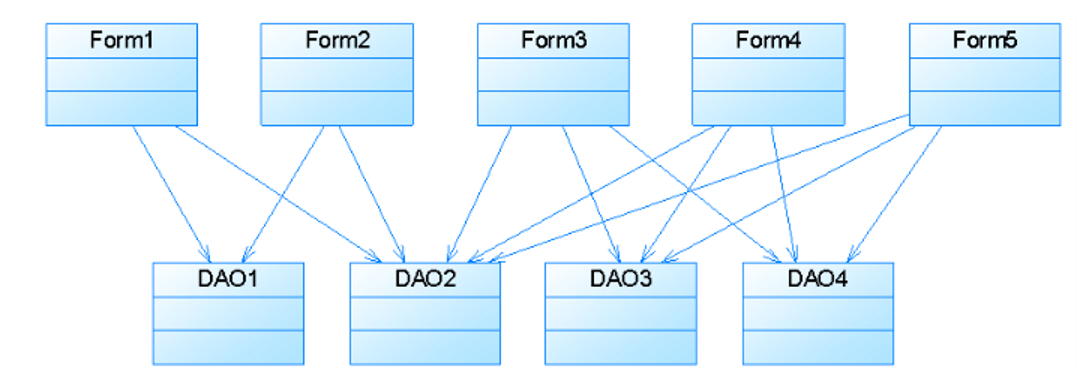
\includegraphics[scale = 0.3]{assets/SoftwareEngineering_b4f96.png}
  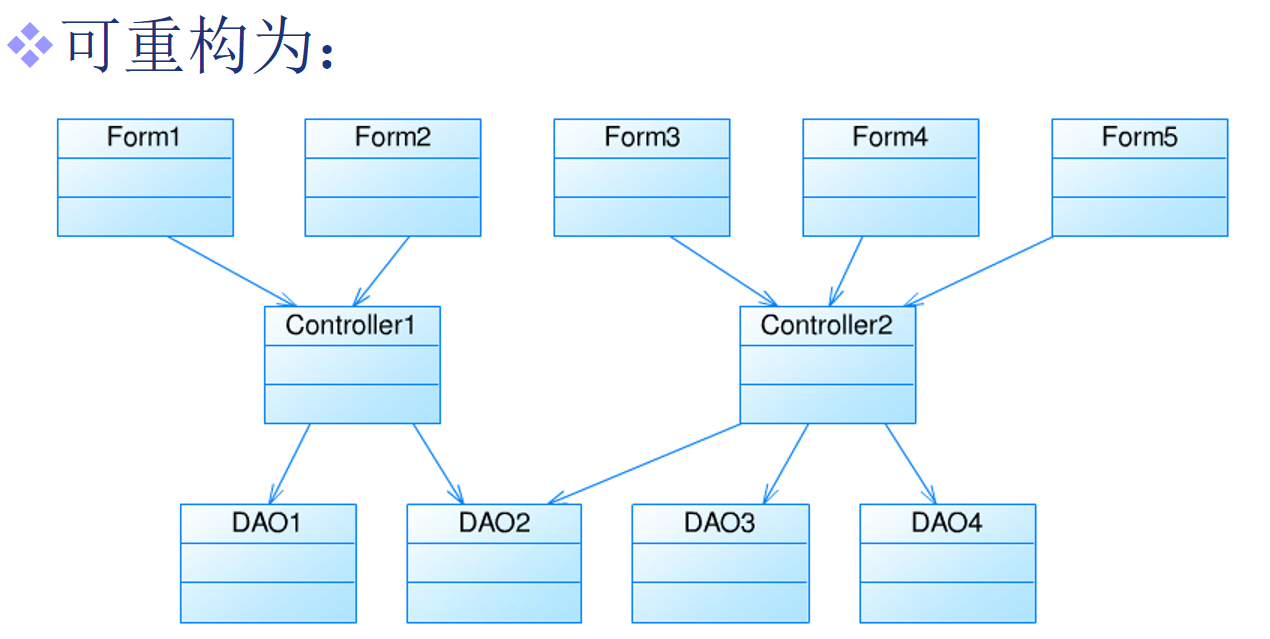
\includegraphics[scale = 0.3]{assets/SoftwareEngineering_5e4f3.png}
\end{figure}

LKP代价:系统增加了一些类

\section{设计模式}
\subsection{背景}
设计模式是90年代以后的重要研究方向,解决软件危机的一些问题

\textbf{模式}一词起源于$<<$建筑的永恒之道$>>$

后来计算机设计模式开创者"四人帮"引入(设计模式-可复用面向对象软件的基础 是设计模式的奠基之作)

\textbf{什么是模式?}模式是指共同问题的解决方案,用于复用

在设计模式之前,代码复用更多体现在代码层面,之后复用技术提高到解决方案的层面上

\subsection{设计模式的分类}
按目的的划分(国外)
\begin{itemize}
  \item 创新型\\
  实例化过程
  \item 结构型\\
  组合类与对象以获得更大的结构
  \item 行为型\\
  涉及算法与对象职责分配问题
\end{itemize}

按粒度划分(国内):
\begin{itemize}
  \item 体系结构模式
  \item 设计模式
  \item 习语(代码模式)
\end{itemize}

\subsection{工厂模式}
工厂模式:类的创建模式

动机:为使用对象,还需要对象的创建与初始化工作,工厂模式承担对象的创建工作,让对象的使用与创建分开来

\begin{itemize}
  \item 简单工作\\
  静态工厂方法模式
  \item 一般工厂方法\\
  多态工厂模式
  \item 抽象工厂模式
\end{itemize}

工厂模式的优点:工厂类是整个模式的关键.包含了必要的逻辑判断,根据外界给定的信息,决定究竟应该创建哪个具体类的对象.通过使用工厂类,外界可以从直接创建具体产品对象的尴尬局面摆脱出来,仅仅需要负责“消费”对象就可以了。而不必管这些对象究竟如何创建及如何组织的.明确了各自的职责和权利,有利于整个软件体系结构的优化。

简单工厂模式通过这种做法实现了对责任的分割。

什么情况下使用工厂模式合适?

涉及的产品相对固定,不适合产品经常发生变化的情况(绝大部分单例使用工厂模式)

\subsubsection{静态工厂模式}
静态工厂是由一个工厂生产所有产品

怎么使用OC原则评价工厂模式?
不满足工厂模式,因为工厂需要修改代码,虽然添加新的子类无需修改其他代码

不存在一种设计模式能解决所有问题

评价一个设计模式往往使用OC原则评价,哪些部分对扩展开放,哪些部分对修改闭合

\subsubsection{一般工厂方法}
若产品经常发生变换,又希望使用工厂模式,怎么改进?多态工厂方法,又叫虚拟构造子模式

怎么改进静态工厂使之满足OC原则?

通过工厂接口把创建工作交给子类,每个产品都有对应的工厂进行生产工作

\subsubsection{抽象工厂模式}
又称工具箱模式,工厂模式中最为抽象, 最具一般性的一种形态

同一组件在不同OS业务功能相同,唯一不同的是底层调用不同(创建工作不同)

如果说多态工厂是单一产品创建,那么抽象工厂就是创建一个产品簇

比如:所有windwos OS组件同一封装,所有Linux 同一封装

\begin{figure}[H]
  \centering
  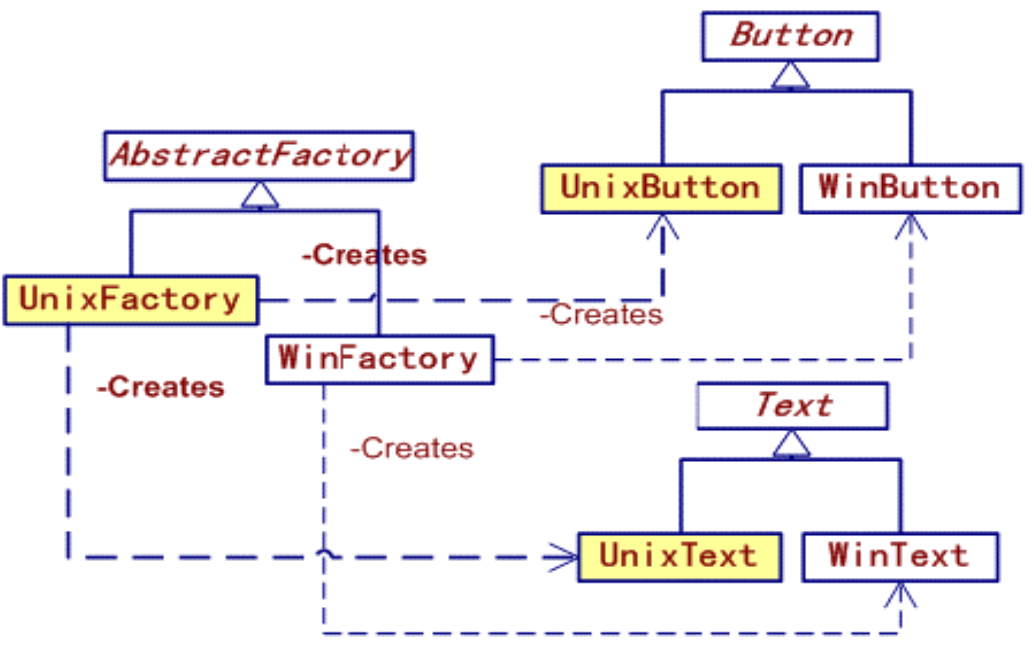
\includegraphics[scale = 0.3]{assets/SoftwareEngineering_e579a.png}
\end{figure}

评价:
\begin{itemize}
  \item 可能增加新的类
  \item 增加新的产品,原来的工行需要增加新产品的创建工作,和静态工厂一样
\end{itemize}

\subsection{策略模式}
策略模式:将一组算法中的每个算法封装到具有共同接口的独立类中,使得他们可以相互替换(一个策略一个类)

\begin{itemize}
  \item 动态地选择一种行为
  \item 一个系统使用的数据不可以让客户端直到
  \item 避免使用难以维护的多重选择语句,体现面向对象设计的概念
\end{itemize}

优点:
\begin{itemize}
  \item 策略模式提供了管理相关的算法族的办法。避免重复的代码。
 \item 策略模式提供了可以替换继承关系的办法。使其不可能动态改变算法或行为。
 \item 使用策略模式可以避免使用多重条件转移语句。
\end{itemize}

缺点:
\begin{itemize}
  \item 客户端必须知道所有的策略类,并自行决定使用哪一个策略类。
 \item 策略模式造成很多的策略类
\end{itemize}

\section{软件测试}

软件测试的目的:为了发现故障,而不是为了证明没有问题

\begin{itemize}
  \item 黑盒测试\\
  测试对象的功能,按对外提供方法,验证输出是否正确
  \item 白盒测试\\
  测试对象的结构
  \item 验证测试\\
  基于概要/详细设计测试
  \item 确认测试\\
  站在用户的角度,基于需求规格说明书测试
\end{itemize}

\subsection{单元测试}
\begin{itemize}
  \item 代码走查(个人)\\
  一般由开发者承担
  \item 代码审查\\
  多个人,更加正规
\end{itemize}

形式化证明技术:主要用于安全性,可靠性项目,时间成本大

继承测试:
\begin{itemize}
  \item 构件测试
  \item 模块测试
\end{itemize}
早期:
\begin{itemize}
  \item 自底向上
  \item 自顶向下
  \item 一次性\\
  同时都测
  \item 三明治\\
  中间往两头
  \item 改进的自顶向下
  \item 改进的三明治
\end{itemize}

自底向上存在的问题:模块往往存在相互调用关系,因此可能存在需要的调用还未被测试

\begin{itemize}
  \item 测试计划
  \item 测试过程:
  \begin{itemize}
    \item 功能测试
    \item 性能测试\\
    在线人数,并发性(按在线人数5\%估算)
    \item 验收测试
    \item 安装测试
  \end{itemize}
  \item 系统测试技术\\
  回归测试:对上次错误进行修正后进行测试,可以全部重新测试,也可以只测试修改的部分
  \item 测试小组
  灰度测试:小范围内测试,逐渐扩大范围,若未发现问题,则替换旧拌饭,否则立刻回退版本
  \item 可靠性,可用性,可维护性,失效严重级别
  \item 验收测试
  初验和终验,类型:
  \begin{itemize}
    \item 验证性测试
    \item alpha 测试
    \item beta测试
    \item 并行测试
  \end{itemize}
\end{itemize}

\section{维护}
维护:生命周期成本最大的阶段

分类:
\begin{itemize}
  \item 改正性\\
  软件初期
  \item 适应性\\
  系统运行环境发生变化
  \item 完善性\\
  后期维护占比重大
  \item 预防性\\
  防止系统性能下降到不可接受的程序
\end{itemize}

重构:
\begin{itemize}
  \item 重新设计
  \item 功能不变
\end{itemize}

再工程:
\begin{itemize}
  \item 正向
  \item 逆向
\end{itemize}

\section{期末复习提纲}
\subsection{考试题型、时间、地点}
闭卷考试,使用答题卡作答

\textbf{时间、地点:}2017-12-27 17周 周三 8:50-10:50 A1501,505 南校区 苏锦钿

\textbf{题型:}
\begin{itemize}
  \item 选择题:$1' \times 20= 20'$
  \item 判断题:$2' \times 10 = 20'$
  \item 简答题:$5' \times 8 = 40'$\\
  比较简单,上课讲过的内容,若记不清楚,可以结合自己的理解填写答案,不要留空
  \item 应用题:$20' \times 1 = 20'$\\
  列需求,进行文字分析,分析用例,涉及用例图,类图等,主要是类图,要求标出类间的关系
\end{itemize}

\subsection{软件工程概述}
\paragraph{什么是软件?}是一系列按照特定顺序组织的计算机数据和指令的集合,包括程序、数据和文档

软件 = 程序 + 数据 + 文档

\paragraph{什么是软件危机, 其内容主要是指什么?}
无统计、准确的答案,自己概括

软件危机:168年提出, 根本原因是软件发展跟不上硬件的发展,硬件发展满足摩尔定律

软件危机有哪些表现?
\begin{itemize}
  \item 软件质量低下
  \item 开发成本高
  \item 可维护性差
  \item 开始时间 超过 预期
\end{itemize}

\paragraph{什么是软件工程?}PP.24

\paragraph{软件工程的目标及其组成部分}PP.41
软件工程的三个要素 , 三个 研究方向
\begin{itemize}
  \item 方法论
  \item 工具
  \item 过程
\end{itemize}

\paragraph{软件 开发方法 的 定义}

\paragraph{好的软件的一些衡量指标} 例如 \textbf{McCall}的质量模型

\begin{itemize}
  \item mcCall的质量模型
  \item 常见的软件质量模型及其对应的指标是什么?
\end{itemize}

\textbf{常用的质量模型指标是什么?并简要介绍}
不要混淆
\begin{itemize}
  \item 可维护性
  \item 可靠性
  \item 可用性
  \item 安全性
\end{itemize}

\subsection{过程和生命周期建模}
\paragraph{什么 是 软件 生命周期?主要 分为 哪些 阶段? 各个阶段 的 主要任务 及 产生 的主要制品?}

\textbf{什么是软件生命周期?}

软件从产生到废弃使用的整个过程

\textbf{分为哪些阶段?}
\begin{itemize}
  \item 可行性分析\\
  可行性分析报告
  \item 需求分析\\
  需求规格说明书
  \item 设计阶段
  \begin{itemize}
    \item 概要设计
    \item 详细设计
  \end{itemize}
  \item 开发
  \item 测试\\
  测试方案
  \item 维护
\end{itemize}

\paragraph{需求分析的定义}

需求分析主要分为
\begin{itemize}
  \item 功能性需求
  \item 非功能性需求
\end{itemize}

需求分析应该站在用户的角度看待问题,而不是从开发者的角度看待问题

\paragraph{典型的软件开发过程模型的特点(优缺点)及要求,特别是原型法、瀑布模型、螺旋模型、增量和迭代等}

\textbf{瀑布模型:}第一个过程模型,重量级模型,通过严格有序的过程明确各个阶段的关系,上一阶段完成才能进行下一阶段

阶段完成的标志是 \textbf{文档是否满足要求}

适合什么场景?适合需求明确,不发生改变的任务

有什么不足?用户最后阶段完成才能拿到产品,才能知道系统张什么样子

瀑布模型提出的背景?解决软件危机

\textbf{螺旋形模型}:考虑风险

\textbf{增量和迭代}:快速成品

增量:增加功能

迭代:完善原有功能

\paragraph{原型法的特点及分类}
\textbf{原型法}:

适合用户需求不明确的场景,分为
\begin{itemize}
  \item 探索型、实验型\\
  一旦明确需求之后,丢弃原型重新开发
  \item 演化型\\
  明确续之后,在原型的基础上进行演化
\end{itemize}

背景:快速建模工具的出现,使得可以快速建立原型

\paragraph{敏捷开发方法和极限编程的特点}这点考试涉及内容不多,了解主要特点即可

敏捷开发方法:体现在文档减少及各阶段流程、规章制度、约束的减少

极限编程:测试先行,是敏捷开发方法的一种

\subsection{计划和项目管理}
\paragraph{了解项目计划和管理的主要内容和常用方法}

\paragraph{软件可行性研究的内容}
可行性论证,包括:
\begin{itemize}
  \item 技术上的可行性
  \item 经济可行性研究
  \begin{itemize}
    \item 项目成本
    \item 项目效益
  \end{itemize}
  \item 对产品而言,市场可行性研究
  \item 法律可行性研究\\
  用户隐私什么的
\end{itemize}

\subsection{获取需求}

\paragraph{了解需求的重要性及需求分析阶段的目标及主要产物}

\paragraph{需求工程包括哪些方面?}
软件成本主要是因为需求阶段,因此,90年代以后,需求分析单独演变成了需求工程

需求工程主要包括:
\begin{itemize}
  \item 需求获取
  \item 需求建模
  \item 需求验证
  \item 需求变更
\end{itemize}

\paragraph{需求的类型:功能需求、非功能需求 或 质量需求 、设计约束 、过程约束}

\paragraph{两种需求文档}:需求定义文档和需求规格说明书

\paragraph{需求规格说明书的主要内容}

\paragraph{常用的需求建模表示方法}ER图、事件跟踪、状态机、Petri网、数据流图、用例图 和 原型法

\subsection{补充材料-UML部分}

\paragraph{UML的作用}:是为软件系统的制造进行描述(specifying)、可视化(visualizing)、构造(constructing) 、 文档化 (dcumenting) 的一种语言

\paragraph{UML中的4+1视图}
\begin{itemize}
  \item 用例图
  \item 设计视图
  \item 进程视图
  \item 实现视图
  \item 分布视图
\end{itemize}

\paragraph{UML的三种扩展机制}:
\begin{itemize}
  \item 构造型 stereotype
  \item 标记值 tagged value
  \item 约束 contraint
\end{itemize}

\paragraph{UML中所包含的10种图形及其各自的作用}

\paragraph{用例图的作用}

\paragraph{用例图的主要构成部分}

\paragraph{类图的主要作用}

\paragraph{了解类之间的各种关系}
\begin{itemize}
  \item 关联
  \item 依赖
  \item 继承或泛化
  \item 组合 / 聚合
\end{itemize}

\paragraph{了解类图的基本建模步骤}

\paragraph{接口和抽象类的定义及各自特点}

\paragraph{交互图的分类}
\begin{itemize}
  \item 顺序图
  \item 协作图
\end{itemize}
这两种图形各自的优缺点???

注意UML2.0中 协作图改称通信图

\paragraph{状态图和活动图各自的作用}注意活动图中泳道的作用

\paragraph{组件图的作用以及组件和结构间的关系}

\paragraph{部署图的作用以及节点的分类}

\paragraph{主要面向对象设计原则及各自的原理}
\begin{itemize}
  \item OCP
  \item LSP原则
  \item DIP
  \item ISP
  \item CARP
  \item LoD
\end{itemize}

\paragraph{设计模式的内容和分类}
按粒度分类:
\begin{itemize}
  \item 体系
  \item 设计
  \item 代码
\end{itemize}

\paragraph{设计模式与面向对象设计之间的关系,特别是OCP原则}

\paragraph{了解常见设计模式的设计思想及其原理,了解如何从OCP的角度进行分析}
怎么样用OC原则评价设计模式的好坏(需求变换会引起代码什么变化)

\subsection{设计系统}
\paragraph{概念设计和技术设计的内容}

\paragraph{好的设计的衡量:内聚和耦合}

\paragraph{常用的内聚和耦合度类型}

哪种内聚类型易导致高内聚

\subsection{测试}
\paragraph{测试的目标和衡量标准}
成功测试的标准:能否找到相应的错误

测试的目的是为了找到错误,而不是为了证明不存在错误

\paragraph{测试的分类(或组织) , 各种类型的测试的主要任务及所依赖的文档}

\paragraph{黑盒测试核白盒测试的思想,了解白盒测试中的基本路径测试等方法}

\paragraph{单元测试的主要内容}

\paragraph{集成测试的类型及主要的测试策略}

\paragraph{确认测试的内容}

\paragraph{了解测试计划的主要内容}

\paragraph{测试系统中的测试过程:}
\begin{itemize}
  \item 功能测试
  \item 性能测试
  \item 验收(或确认)测试
  \item 安装测试
\end{itemize}
以及他们的内容

\subsection{系统维护}
\paragraph{维护活动的类型}
\begin{itemize}
  \item 改正性
  \item 适应性
  \item 完善性
  \item 预防性
\end{itemize}

\paragraph{各种维护活动的主要内容和目标}

\paragraph{软件再生:}
\begin{itemize}
  \item 文档重构
  \item 重组
  \item 逆向工程
  \item 再工程
\end{itemize}

以及他们各自的内容和含义

\subsection{其他}
\paragraph{了解产品评估的几种方法}
\begin{itemize}
  \item 特征分析
  \item 调查
  \item 案例研究
  \item 正式的试验
\end{itemize}

\paragraph{了解几种主要的产品质量模型}
\begin{itemize}
  \item Boehm的模型
  \item ISO 9126
  \item Dromey模型
\end{itemize}

\paragraph{了解常用的过程评估模型}
\begin{itemize}
  \item CMM
  \item SPICE
  \item CMMI
  \item ISO 9000
\end{itemize}

\paragraph{了解软件工程与计算机科学的关系}

\paragraph{软件工程的主要研究内容及面临的一些主要问题}

\end{document}
